\documentclass[12pt]{article}

% Set margins
\usepackage[margin=1in]{geometry}
% Remove paragraph indentation
\setlength{\parindent}{1\baselineskip}
\setlength{\parskip}{0.5\baselineskip}

\usepackage{amsmath}
\usepackage{amssymb}
\usepackage{amsfonts}
\usepackage{hyperref}
\usepackage{amsthm}
\usepackage{amscd}
\usepackage{tikz-cd}
\usepackage{enumitem}
\usepackage{mathrsfs}
\usepackage{biblatex}
\usepackage{mdframed}
\addbibresource{refs.bib}

% Define a new style with italicized title
\newtheoremstyle{defstyle} % name
    {12pt}        % Space above
    {12pt}        % Space below
    {\upshape}  % Body font
    {}           % Indent amount
    {}          % Theorem head font
    {.}         % Punctuation after theorem head
    {.5em}      % Space after theorem head
    {\textbf{\thmname{#1}\thmnumber{ #2}} (\textit{\thmnote{#3}})}  % Theorem head spec

\newtheoremstyle{remarkstyle} % name
    {12pt}        % Space above
    {12pt}        % Space below
    {\upshape}  % Body font
    {}           % Indent amount
    {}          % Theorem head font
    {.}         % Punctuation after theorem head
    {.5em}      % Space after theorem head
    {\textbf{\thmname{#1}\thmnumber{ #2}}}  % Theorem head spec


\usepackage{amsthm}
\theoremstyle{defstyle}
\newtheorem{theorem}{Theorem}
\newtheorem{definition}{Definition}
\newtheorem{example}{Example}

\theoremstyle{remarkstyle}
\newtheorem{lemma}[theorem]{Lemma}
\newtheorem{proposition}[theorem]{Proposition}
\newtheorem{remark}{Remark}
\newtheorem{corollary}{Corollary}
\newtheorem{theoremr}{Theorem}

\numberwithin{equation}{section}
\numberwithin{definition}{section}
\numberwithin{corollary}{section}
\numberwithin{theorem}{section}
\numberwithin{theoremr}{section}
\numberwithin{remark}{section}
\numberwithin{example}{section}

% Tocloft package for table of contents customization
\usepackage{tocloft}
\setcounter{tocdepth}{1} % Set depth to show only sections in table of contents

\usepackage{algorithm, algpseudocode, subfig}
\usepackage{graphicx}% Include figure files
\usepackage{dcolumn}% Align table columns on decimal point
\usepackage{bm}% bold math


% Custom command definitions
\newcommand{\ra}{\rangle}
\newcommand{\la}{\langle}
\newcommand{\df}{\dfrac}
\newcommand{\hb}{\hbar}
\newcommand{\intf}{\int_{-\infty}^\infty}
\newcommand{\ang}[1]{\left\la #1 \right\ra} % \lang{H} = <H>
\newcommand{\pd}[1]{\partial_{#1}} % Shorthand for partial derivatives
\newcommand{\R}{\mathbb R}
\newcommand{\EL}{\mathbb L}
\newcommand{\mbb}{\mathbb}
\newcommand{\Exp}{\mbb E}
\newcommand{\D}{\mathcal D}
\newcommand{\p}{\partial}    
\newcommand{\mbf}{\mathbf}    
\newcommand{\xra}{\xrightarrow}
\newcommand{\X}{\mathfrak{X}}
\newcommand{\calD}{\mathcal D}
\newcommand{\Der}{\mathrm{Der}}
\newcommand{\Lie}{\mathcal L}
\newcommand{\mrm}{\mathrm}
\newcommand{\prf}{\textit{Proof: }}
\newcommand{\mfk}{\mathfrak}
\newcommand{\La}{\mathfrak{a}} % a for Lie algebra
\newcommand{\supp}{\mathrm{supp}}
\newcommand{\Hom}{\mathrm{Hom}}
\newcommand{\End}{\mathrm{End}}

\newcommand{\sR}{\mathscr{R}}
\newcommand{\sE}{\mathscr{E}}
\newcommand{\fR}{\mathfrak R}
\newcommand{\N}{\mathbb N}
\newcommand{\Normal}{\mathcal N}
\newcommand{\tr}{\mathrm{tr}}
\newcommand{\mca}{\mathcal}
\newcommand{\Hi}{\mca H}
\newcommand{\B}{\mca B}
\newcommand{\K}{\mca K}
\newcommand{\C}{\mathbb C}
\newcommand{\Her}{\mathrm{Her}}
\newcommand{\Pa}{\mca P}
\newcommand{\Z}{\mathbb Z}
\newcommand{\Pos}{\mathrm{Pos}}
\newcommand{\br}{\mbf r}

% Commands for multilinear algebra
\newcommand{\sgn}{\mathrm{sgn}}

% Labeled, aligned, equation
\newcommand{\leqalign}[2]{
\begin{equation}\begin{aligned}\label{#1}
#2
\end{aligned}\end{equation}}
\newcommand{\malign}[1]{
\[\begin{aligned}
#1
\end{aligned}\] 
}
\setlist[enumerate]{itemsep=0pt, topsep=0pt, partopsep=0pt}
\setlist[itemize]{itemsep=0pt, topsep=0pt, partopsep=0pt}



\begin{document}

\title{Quantum Mechanics}
\author{Nicholas Lyu}
\date{\today}
\maketitle


These notes are for the fall 2023 iteration of Harvard's second-semester 
undergraduate quantum mechanics, Physics 143b, taught by Sonia Paban. 
The course includes a brief introduction to path integrals, 
followed by perturbation theory applied 
to hydrogen energy levels, then quantum dynamics, WKB approximation, 
scattering, and density operators. 

These notes deviate from the course material by 
\begin{itemize}
    \item a section on symmetry and conservation laws, adapted from Griffiths. 
    \item an interaction-picture explanation of time-dependent perturbation theory, 
        adapted from MIT's online lecture notes. 
    \item the adiabatic theorem from Weinberg's \textit{Lectures on Quantum Mechanics}. 
    \item does not include density operators. 
\end{itemize}
A note on notations: $d/dx, \partial /\partial x$ are abbreviated $d_x, \pd x$. 
Summation over a free index which does not appear on the left hand side are occasionally 
omitted to reduce clutter. Function arguments are occasionally integerchanged with subscripts 
to reduce clutter. 

\tableofcontents
\pagebreak
\section{Path Integrals}
\subsection{Gaussian Integrals}
A single-variable Gaussian integral may be evaluated by a change into spherical coordinates: 
\begin{equation}
    G(a)=\intf dx\, \exp(-ax^2)=\sqrt{\df \pi a}
\end{equation}

More generally, we may consider a general Gaussian integral for a positive definite $n\times n$ matrix $A$
and offset $\omega$. 
\begin{equation}\label{eqn:real_multivariable_gaussian}
    \intf (dx_1\cdots dx_n)\, \exp\left(-x^TAx + \omega^Tx\right)=
    \exp\left(\df 1 4 \omega^TA^{-1}\omega\right)\sqrt{\df {\pi^N}{\det A}}
\end{equation}
The integral is evaluated by diagonalizing $A$ and completing the square, as below:
\[x^TAx - \omega^Tx = \left(x - \df{A^{-1}\omega}2\right)^TA\left(x-\df{A^{-1}\omega}2\right) 
- \df 1 4 \omega^TA^{-1}\omega\]

We may also consider integrating imaginary, oscillating exponentials: 
\begin{itemize}
    \item Put in by hand a convergence factor \(\exp(-\delta x^2)\), then take $\delta\to 0$
    \item Perform the change of variables $x'=\sqrt{-i\alpha} x$
\end{itemize}
The following integrals from \href{https://en.wikipedia.org/wiki/Common_integrals_in_quantum_field_theory}{Wikipedia}
are helpful:
\begin{equation}\label{eqn:complex_multivariable_gaussian}
\begin{aligned}
    \intf d^nx\, \exp\left(-\df 1 2x^T A x + \omega^Tx \right) &= \sqrt{\df{(2\pi)^n}{\det A}}\exp
        \left(\df 1 2 \omega^T A^{-1} \omega\right)
    \\ 
    \intf d^nx\, \exp\left(-\df 1 2x^T A x + i\omega^Tx \right) &= \sqrt{\df{(2\pi)^n}{\det A}}\exp
    \left(-\df 1 2 \omega^T A^{-1} \omega\right)
    \\ 
    \intf d^nx\, \exp\left(-\df i 2x^T A x + i\omega^Tx \right) &= \sqrt{\df{(2\pi i)^n}{\det A}}\exp
    \left(-\df i 2 \omega^T A^{-1} \omega\right)
\end{aligned}
\end{equation}

\subsection{Propagator}
Recall that in Lagrangian mechanics, the Lagrangian \(\mathcal L(q, \dot q, t)\) is usually 
associated with \(T-V\). Based on the Lagrangian, one may define the action functional as below, where \(t_1, t_2\) 
may be omitted if clear from context. 
\[S_{t_1, t_2}[q]=\int_{t_a}^{t_b} \mathcal L(q(t), \dot q(t), t)\]
\begin{example}[Classical free particle]
    Recall a free point particle with 
    \[\mathcal L = m\dot x^2/2\]
    The Lagrangian e.o.m and the resulting classical path are
    \[m\ddot x = 0\implies x_{\mathrm{cl}}(t)=\df{x_b-x_a}{t_b-t_a}(x-t_a)+x_a\]
    The corresponding classical action is 
    \[S[x_{\mathrm{cl}}] = 
        \int_{t_a}^{t_b} dt\, \df 1 2 m \left(\df{x_b-x_a}{t_b-t_a}\right)^2
        = \df{m(x_b-x_a)^2}{2(t_b-t_a)}\]
\end{example}

The theorem below shows how the path integral formulation quantum mechanics is based 
classical Lagrangian mechanics. The following theorem demonstrates its relation to 
the Hamiltonian formulation of quantum mechanics.

\begin{definition}[propagator]
    Given the Lagrangian for a system, its \textbf{propagator}, or \textbf{kernel}, is 
    the following integral over all paths \(q\) such that \(q(t_a)=x_a, q(t_b)=x_b\)
    \begin{equation}\label{eqn:def_propagator}
        K(x_b, t_b, x_a, t_a)=\int D[q]\, \exp\left(\df i \hbar S[q]\right)
        =\int D[q]\, \exp\left(\df i \hbar \int_{t_a}^{t_b}dt\, \mathcal L(q(t), \dot q(t), t)\right)
    \end{equation}
\end{definition}
    
\begin{theorem}[path integral formulation]
    The kernel satisfies \[K(x_b, t_b, x_a, t_a)=\ang{x_b, t_b|x_a, t_a}\]
    In other words, the Hamiltonian and Lagrangian formulation of quantum mechanics are 
    compatible in the following way (assuming a time-indepent Hamiltonian)
    \begin{equation}\label{eqn:propagator_hamiltonian}
        \int D[q]\, \exp\left(\df i \hbar \int_{t_a}^{t_b}dt\, \mathcal L(q(t), \dot q(t), t)\right)
        = \ang{x_b\left|\exp\left(-\df i \hb (t_b-t_a)H\right)\right|x_a} 
    \end{equation}
\end{theorem}

\begin{remark} 
    Several remarks are in order:
    \begin{itemize}
    \item 
        Every path $q$ contributes a factor with absolute value $1$: contributions only differ in phase. 
        Conceptually, the first-order endpoint-preserving variations vanish at the classical path (which satifies the 
        Lagrangian equations of motion), resulting in in-phase contributions, while those paths far from 
        the classical one are easily out of phase.
    \item 
        The destructive interference far away from the classical path relies on the large value of $\Delta S / \hb$. 
        This qualifies how quantum mechanics degenerates to classical mechanics in the limit $\hb\to 0$, or when action 
        scales are large when compared to $\hb$, as in the case for most macroscopic systems. 
    \item 
        Should we choose to describe our system as an evolving field $\Psi(x, t)$ instead of a path $q(t)$,
        the path-integral formulation generalizes in a straightforward way:
        \[\int D[\Psi]\exp\left(\df i \hb \int d^4x\, \mathcal L(\Psi, \dot \Psi, t)\right)\]
    \item 
        We're assuming spinless particles. 
        There are subtle ties to commutativity here. 
    \item 
        The position basis in $K(b, a)=\la x_b|U(t_b-t_a)|x_a\ra$ is special. We cannot use the Lagrangian 
        should we choose a different basis for the propagator.  
    \end{itemize}
\end{remark}

The propagator $K$ determines the dynamics. We take the basis $|x, t\ra$ 
and view the system state as defined on the whole space-time, with time evolution via varying $t$: 
\begin{equation}\begin{aligned}\label{eqn:propagator_evolution}
    \psi(x, t) 
        &= \ang{\psi|x, t} = \la \psi|{\sum}_{x'}\la x, t|x', t_0\ra |x', t_0\ra  \\ 
        &= {\sum}_{x'}K(x, t, x', t_0)\la \psi|x', t_0\ra \\ 
        &= {\sum}_{x'}K(x, t, x', t_0)\psi(x', t_0)
\end{aligned}\end{equation}
Alternatively, assuming a time-invariant Hamiltonian and an energy basis $\{|n, t\ra\}$
\begin{equation}\begin{aligned}\label{eqn:propagator_energy_eigenstates}
    K(x, t, x', t') 
        &= \la x, t|x', t'\ra \\ 
        &= {\sum}_n \la x, t'|n\ra \la n|x, t\ra \\ 
        &= {\sum}_n \exp\left(-\df i \hb E_n(t-t')\right)\psi_n^*(x)\psi_n(x')
\end{aligned}\end{equation}
The propagator satisfies the Schrodinger equation: fixing $x', t'$ (recall equation~\ref{eqn:propagator_hamiltonian})
\begin{equation}
    i\hb \pd t K(x, t, x', t') = H_t K(x, t, x', t')
\end{equation}
\begin{remark}
    The dynamics of the system is captured by a one-parameter family of unitaries $U_t$, 
    obtained by integrating the exponential of the Hamiltonian (or computing the Schrodinger 
    equation), which send initial states $|\psi_0\ra$ to $|\psi_t\ra$. 
    The propagator is simply the representation of this unitary in the position basis. 
    To see why, recall the action of a linear operator $A$ with matrix representation $(A_{ij})$ 
    in a finite-dimensional Hilbert space 
    \[ 
        (Av)_i = \sum_j A_{ij} v_j 
    \] 
    The matrix element representation $A_{ij}$ may be viewed instead as a map $A(i, j)=A_{ij}$ 
    and the states similar maps $v(j) = v_j$. 
    \[ 
        (Av)(i) = \sum_j A(i, j)v(j)
    \] 
    The direct analogue of this in infinite-dimensional Hilbert space is to replace summing 
    over the discrete index $j$ with integration over a continuous variable $x$ 
    \[ 
        \psi_t(x) = (U_t\, \psi_0)(x) = \int K_{0\to t}(x, x')\psi_0(x')\, dx' 
    \] 
\end{remark}

\subsection{Integration over paths}
Consider the following method of parameterizing all possible paths $(x_a, t_a)\to (x_b, t_b)$. 
Discretize time by units of $\epsilon$: let $t_0=t_a, t_N=t_b, N\epsilon = t_b-t_a$, and $t_{j+1}=t_j+\epsilon$. 
\begin{equation}
    K(b, a)\sim \lim_{\epsilon \to 0, N\epsilon = \Delta t}\int\cdots \int (dx_1\cdots dx_{N-1}) \exp\left(\df i \hb S[q(x_1\cdots x_{N-1})]\right)
\end{equation}
Note that $x_0, x_N$ are fixed, so they are not variables to be integrated. 
Under this parameterization, the values $\{x_1\cdots x_{N-1}\}$ parameterizes a path $q$ under the following substitution:
\begin{equation}\begin{aligned}
    S[q]&=\int_{t_a}^{t_b}\mathcal L(q, \dot q, t)\, dt = \sum_{j=0}^{N-1}\mathcal L\left(x_i, \df{x_{i+1}-x_i}{\epsilon}, t\right)
\end{aligned}\end{equation}

\subsection{Separable Lagrangian}
Let $q_{\mathrm{cl}}$ denote the classical path satisfying Euler-Lagrange equations. 
Consider the following quantity for an endpoint-preserving perturbation $\eta$ and time-invariant Lagrangian: 
\begin{equation}
\begin{aligned}
    \mathcal L(q_{\mathrm{cl}}+\epsilon \eta, \dot q_{\mathrm{cl}}+\epsilon \dot \eta)  
    &= \sum_{n=1}^\infty \df 1 {n!} \left[\epsilon \left(\eta \pd q + \dot \eta \pd{\dot q}\right)\right]^n \mathcal L(q_{\mathrm{cl}}, \dot q_{\mathrm{cl}}, t) \\ 
    &= \left[1 + 
        \epsilon (\eta \pd q + \dot \eta \pd{\dot q}) + 
        \epsilon^2\left(\eta^2 \pd{q}^2 + 2(\eta \pd q)(\dot \eta d_{\dot q}) + \dot \eta^2 \pd{\dot q}^2\right)
        +O(\epsilon^3)\right]\mathcal L_{\mathrm{cl}}
\end{aligned} 
\end{equation}
The zeroth-order term denotes the classical action, the first-order term vanishes by the 
Euler-Lagrange equations, and the second-order terms preserve the quadratic coefficients. 

\begin{theorem}[quadratic Lagrangians are separable]
    For quadratic Lagrangians of the form 
    \[\mathcal L(q, \dot q, t)=Aq^2+B\dot q^2\]
    Both the Lagrangian and the action separate linearly by classical paths 
    \begin{equation}\begin{aligned}
        \mathcal L(q_{\mathrm{cl}} + \eta, \dot q_{\mathrm{cl}} + \dot \eta) &= 
            \mathcal L(q_{\mathrm{cl}}, \dot q_{\mathrm{cl}}) + \mathcal L(\eta, \dot \eta) \\ 
        S[q_{\mathrm{cl}}+\eta] &= S[q_{\mathrm{cl}}] + S[\eta]
    \end{aligned}\end{equation}
\end{theorem}

\begin{theorem}[propagator for separable Lagrangian]
    When the Lagrangian separates, the propagator in equation~\ref{eqn:def_propagator} takes the following form. 
    The path integral over $\eta$ is agnostic towards $x_a, x_b$ and only depends on $t_b-t_a$ since the Lagrangian 
    is time-invariant. 
    \[\begin{aligned}\label{eqn:separable_propagator}
        K(x_b, t_b, x_a, t_a)&=\int D[q]\, \exp\left(\df i \hbar S[q]\right) 
        =\int D[\eta]\, \exp\left(\df i \hbar S[q_{\mathrm{cl}}+\eta]\right) \\ 
        &= \exp\left(\df i \hb S_{\mathrm{cl}}\right) \int D[\eta]\, \exp\left(\df i \hbar S[\eta]\right)
        =A(t_b-t_a)\exp\left(\df i \hb S_{\mathrm{cl}}\right)
    \end{aligned}\]
\end{theorem}

\begin{example}[free particle]
    Recall a free particle has Lagrangian $\mathcal L(x, \dot x)=\df 1 2 m \dot x$. 
    \begin{equation}
        K(x, t, x', t') = \sqrt{\df m {2\pi i \hbar \Delta t}}\exp\left(\df{im(x-x')^2}{2\hb \Delta t}\right)
    \end{equation}
    Note the appearance of classical action in the spatially dependent exponential term. 
\end{example}

\begin{example}[simple harmonic oscillator]
    Consider the following Lagrangian 
    \[L=\dfrac {m \dot x^2}{2} - \dfrac{m \omega^2}{2}x^2\]
    The corresponding classical action is 
    \[
        S_{\mathrm{cl}}=\frac{m \omega}{2 \sin(\omega \Delta t)}   \left(\left(x_a^2+x_b^2\right) \cos (\omega  \Delta t)-2 x_a x_b\right)
    \]
    Recalling the simple Harmonic oscillator solution are all real and of the following form 
    \[\psi_n(x)=\dfrac 1 {\sqrt{2^nn!}}\left(\dfrac{m\omega}{\pi \hbar}\right)^{1/4}\exp\left(-\dfrac{m\omega x^2}{2\hbar}\right) 
        H_n \left(\sqrt{\dfrac{m\omega}{\hbar}x}\right)\]
    Perform this substitution and invoke equation~\ref{eqn:propagator_energy_eigenstates}
    \[
        \sqrt{\dfrac{m\omega}{\hbar}}x_a\mapsto \xi, \sqrt{\dfrac{m\omega}{\hbar}}x_b\mapsto \eta
    \]
    \[ 
        K=\sqrt{\dfrac{m\omega}{2\pi \hbar i \sin \omega \Delta t}}
            \exp \left(\dfrac 1 2 (\xi^2+\eta^2)-\dfrac{\xi^2+\eta^2 - 2\xi\eta \exp(-i\Delta t \omega)}{1-\exp(-2i\Delta t\omega)}\right)
    \]
    The exponential term is the exponential of the classical action. 
    \begin{equation}
        K(b, a)=\sqrt{\dfrac{m\omega}{2\pi \hbar i \sin \omega \Delta t}}\exp\left(\dfrac i \hbar S_\mathrm{cl}\right)
    \end{equation}
\end{example}


\section{Symmetry, Conservation Laws, and Selection Rules}
\subsection{Operators in quantum theory}
\subsubsection{Fundamental opertors}
The fundamental operators in quantum theory are $x, p$ with 
\[ 
    (x\, \psi)(x) = x\psi(x), \quad (p\, \psi)(x) = -i\hb \pd x
\] 
They give rise to the canonical commutation relation 
\[ 
    [x, p] = i\hb 
\] 
This commutation relation gives rise to vector operator's commutation relations. 
The momentum operator may be conveniently memorized as using $-\pd x$ to effect 
translation in $x$, using $i$ to keep it skew-Hermitian, using $\hb$ for units. 

\subsubsection{Ladder operators}
For a harmonic oscillator Hamiltonian 
\[ 
    H = \df 1 {2m} \left[p^2 + (m\omega x)^2\right]
\] 
The raising and lowering opperators of interest are 
\[ 
    a_\pm = \df 1 {\sqrt{2\hb m \omega}}\left(\mp i p + m\omega x\right)
\] 
They are conjugates of each other and obey the commutation relations 
\[ 
    [a_-, a_+] = 1, \quad H = \hb \omega \left(a_+a_- + \df 1 2\right)
\] 
We can in turn express $x, p$ in terms of the ladder operators 
\[ 
    x = \sqrt{\df{\hb}{2m\omega}}(a_+ + a_-), \quad p = i \sqrt{\df{\hb m \omega}{2}}(a_+ + a_-)
\] 
Number operator $n$ is defined by $n = a_+a_-$. We conveniently have (operator on left side) 
\[ 
    n\psi_n = n\psi_n, \quad a_+\psi_n = \sqrt{n+1}\psi_{n+1}, \quad a_-\psi_n = \sqrt n \psi_{n-1}
\] 

\subsubsection{Vector operators}
The fundamental commutation relations for vector operators are 
\[ 
    [V_x, V_y] = i\hb V_z; \quad [V_y, V_z] = i\hb V_x; \quad [V_z, V_x] = i\hb V_y 
\] 
We can define $V^2 = V_x^2 + V_y^2 + V_z^2$, then $[V, V^2]=0$. 
We can also define ladder operators 
\[ 
    V_\pm = V_x \pm i V_y 
\] 
They obey the commutation relations 
\[ 
    [V^2, V_\pm] = 0, \quad [V_z, V_\pm] = \pm \hb V_\pm
\] 
Fix an eigenspace of $L^2$ with eigenvalue $\hb^2l(l+1)$ with 
dimension $2l+1$, where $l$ can be an integer or half-integer.
In this eigenspace, 
\[ 
    V_z = \hb \begin{pmatrix}
        l \\ & l-1 \\ &&\ddots \\ &&&-l 
    \end{pmatrix}, \quad
    L_x = \df 1 2 (V_+ + V_-), \quad 
    L_y = \df i {2}(V_- - V_+)
\] 
Here the representations of $V_\pm$ are shifted diagonals of $\hb$. 

\subsection{Transformation}
We first formally consider transformations acting on states. 
\begin{definition}[translation operator]
    We define its action on $\psi(x)$ as 
    \[T(a)\psi(x)=\psi(x-a)\]
    This definition characterizes the action of $T(a)$ on the positional 
    representation of $|\psi\ra$. In terms of states themselves, the translation 
    operator satisfy, for $|\psi'\ra =T(a)|\psi\ra$
    \[\la \psi'|x\ra = \la \psi|x-a\ra\]
\end{definition}
\begin{definition}[parity operator]
    The parity-inverted state $|\psi'\ra = \Pi |\psi\ra$ satisfies 
    \[\ang{\psi'|r} = \ang{\psi'|-r}\]
    Here $|r\ra$ may be generally understood as a 3d positional basis. 
    Represented spherically:
    \[\Pi \psi(r, \theta, \phi) = \psi(r, \pi - \theta, \phi + \pi)\]
\end{definition}
\begin{proposition} For hydrogenic orbitals, 
    $\Pi \psi_{nlm}(r, \theta, \phi) = (-1)^l\psi_{nlm}(r, \theta, \phi)$
    We only need consider the angular part. Recall
    $Y_l^m(\theta, \phi)\propto P_l^m(\cos\theta)\exp(im\phi)$, 
    and $\cos(\pi - \theta)=-\cos\theta$.
\end{proposition}

\begin{definition}[$z$-rotation operator]
    The rotation operator which effects counterclockwise rotation about the 
    $z$-axis by $\varphi$ is 
    \[ 
        R_z(\varphi)\psi(r, \theta, \phi)=\psi(r, \theta, \phi - \varphi)
    \] 
\end{definition}
Transformations, since they map states to states, must be unitary. 
They are effectively a basis permutation. For example, translation effects the 
basis change $|x\ra \mapsto |x-a\ra$. One may view this via the equivalence between 
sliding our state to the right, and sliding the spatial axis to the left while 
following the center of the axis. By unitarity $T^\dag = T^{-1}$. 

Apart from considering the effect of $T$ on $|\psi\ra$,
define its application on an operator $O$ such that expectation values of 
$O$ w.r.t. $T|\psi\ra$ agrees with that of $T(O)$ w.r.t. $|\psi\ra$. This motivates 
the following definition. 
\begin{definition}[operator transformation, invariance]
    The effect of transforming operator $O$ by $T$ is 
    $T(O)=T^\dag O T=T^{-1}OT$. It follows that $O$ is invariant under $T$ if $[O, T]=0$.
    \begin{equation}
        \la \psi|T^\dag OT|\psi\ra = \la \psi|T(O)|\psi\ra \implies T(O)=T^\dag OT
    \end{equation}
\end{definition}

\subsection{Observables and transformations}

Recall that $p = -i\hb \pd x$. Assuming that $\psi(x)$ may be expanded as a power-series.  
\begin{equation}\begin{aligned}\label{eqn:momentum as exponential}
    T(a)\psi(x)&=\psi(x-a)=\sum_{n=0}^\infty \df{(-a)^n}{n!}\pd x^n\psi(x)  \\ 
                &= \sum \df 1 {n!} \left(\df{-ia}{\hb}(-ih\pd x)\right)^n \psi(x)
\end{aligned}\end{equation}

\begin{definition}[exponential of an operator]
    We define the exponential of a Hermitian operator as a power-series, 
    with multiplication denoting composition
    \begin{equation}
        \exp\left(\alpha O\right) = \sum_{n=0}^\infty \df 1 {n!} (\alpha O)^n
    \end{equation}
    This definition is made precise by the formulation of Lie group and Lie algebra, 
    its main property of interest is 
    \begin{equation}
        \pd \alpha \exp(\alpha O) = \alpha \exp(\alpha O)
    \end{equation}
\end{definition}
\begin{definition}[observables generate transformation]
    We say that a Hermitian observable $O$ generates a one-parameter family of 
    transformations $T(a), a\in \R$ if 
    \begin{equation} 
        T(a)=\exp\left(-\df {i a}\hb O\right)
    \end{equation}
\end{definition}
Equation~\ref{eqn:momentum as exponential} shows that momentum generates axial translation. 

More generally, consider a (partial) basis $\{|o\ra\}$ corresponding to the eigenstates of an observable $O$ 
and let $\psi(o)=\la \psi|o\ra$. The basis is partial in the sense that it is the basis of 
one of possibly many components of the tensor product Hilbert space (e.g. position and spin). 
Note that $\psi(o)$ may be a state!
Define the effect of the unitary transformation $T_o(a)$ by $|o\ra \mapsto |o-a\ra$. 
Assuming that $\psi(o)$ may be expanded as a power series in terms of $o$. 
\begin{equation}
    \psi(o-a)=T_o(a)\psi(o)=\sum_{n=0}^\infty \df 1 {n!} ((-a)\, \pd o)^n \psi(o)
    =\exp\left(-a\,\pd o\right)\psi(o)
\end{equation}
Every unitary $T(a)$ is the complex exponential of a Hermitian $O$ which provides the 
phase factors for the eigenvalues of the unitary. We also have the freedom to choose $O$ 
up to a phase scaling factor $\alpha$ with both free value and unit: 
\begin{equation}\label{eqn:transformation_exponential}
    T(a)=\exp\left(\df i \alpha Q(a)\right)=\exp\left(-a\, \pd o\right)\implies Q(a) 
    = a Q = a (i\alpha \, \pd o)
\end{equation}

\begin{remark}
    Equation~\ref{eqn:hermitian_exponential} provides another perspective: 
    each Hermitian $Q$ defines an infinitesimal transformation $\left(1 + ia Q/N\right)$ when $N\to \infty$. 
    This operator is unitary up to a quadratic order:
    \begin{equation}\label{eqn:hermitian_exponential}
        \left(1 + ia Q/N\right)^\dag \left(1 + ia Q/N\right)
        =1+O(1/N^2)
    \end{equation}
    The cumulative action of applying $\left(1 + ia O/N\right)$ for $N$ times is $\exp(ia Q)$
\end{remark}
Returning to equation~\ref{eqn:transformation_exponential}, 
$\pd o$ effects the change $|o\ra\mapsto |o+do\ra$, so we choose $\alpha = -1/\hb$.
\begin{theorem}[Hamiltonian generates time translation] $\exp\left(-i H t/\hb\right)|t_0\ra = |t_0-t\ra$

    \textit{Proof:} this statement is equivalent to Schrodinger's equation. 
    \[ 
        \pd t|\psi\ra = -\df i \hb H|\psi\ra
    \] 
\end{theorem}

\begin{definition}[complete set of compatible observables (CSCO)]
    \label{def:csco}
    A set of Hermitian observables $\{O_j\}$ over a Hilbert space is 
    compatible if they pairwise commute, and complete if for every 
    set of eigenspaces $\{\mathcal S_{O_j, \lambda_k}\}$, their intersection 
    has dimension at most $1$. 
\end{definition}
\begin{example}[CSCO for central potential]
    For any Hamiltonian $H$ which commutes with $L$, the set $H, L_z, L^2$ is 
    a complete set of compatible observables. 
    They pairwise commute and $E_n, l, m$ uniquely determine an eigenstate. 
\end{example}



\subsection{Symmetry and conservation}
The key idea of this section is the diagram below. 
\begin{center}\begin{tikzcd}[row sep=huge, column sep=10em]
    \text{Transformation } T 
    \arrow[r, leftrightarrow, "T=\exp(-iO\lambda/\hbar)"]
    \arrow[d, leftrightarrow, swap, "{[H, T(a)]=0}"]
    & \text{Observable $O$} 
    \arrow[d, leftrightarrow, "{d_t\Pr[O=o, t]=0}"]
    \\
    \text{Symmetry} \arrow[r, leftrightarrow] & \text{Conservation}
\end{tikzcd}\end{center}


A system is defined by its time-evolution, which is defined by its Hamiltonian. 
We first establish the connection between transformation and symmetry. 
\begin{definition}[continuous symmetry]
    A system with Hamiltonian $H$ has continuous symmetry with respect to a family 
    of transformations $T(a)$, parameterized by $a\in \R$, if 
    \[ 
        \forall a\in \R, [H, T(a)] = 0
    \] 
\end{definition}

Transformations biject with observables, up to a constant factor. 
We show that continuous symmetry is equivalent to 
the conservation of an observable. 
\begin{theorem}[conservation is equivalent to commutativity] 
    The probability distribution for observating different values of a Hermitian $O$ 
    is conserved if and only if $[H, O] = 0$.

    \textit{Proof:} suppose $[H, O]=0$, then the energy eigenstates $|n\ra$ are also eigenstates of 
    $O$.
    \[ 
        |\psi_0\ra = \sum c_n |n\ra\implies \Pr[O=o_n, t=0] = |c_n|^2
    \] 
    Under time evolution, the probability distribution is unchanged 
    \[ 
        |\psi_t\ra = \sum \exp\left(iE_n t/\hb\right) c_n |n\ra\implies 
        \Pr[O=o_n, t] = |\exp\left(iE_n t/\hb\right) c_n|^2=|c_n|^2
    \]
    Conversely, distribution conservation in particular implies $\la O\ra = 0$ (Ehrenfest's theorem):
    \[ \begin{aligned}
        d_t\la O\ra 
            &= d_t\ang{\psi|O|\psi} \\ 
            &= \left(d_t|\psi\ra\right)^\dag O|\psi\ra + \left(O|\psi\ra\right)^\dag d_t|\psi\ra + \pd t O \\ 
            &= \df i \hb \ang{[H, O]}
    \end{aligned}\] 
    The expectation value vanishes for all $|\psi\ra$, so $[H, O]=0$. 
\end{theorem}

\begin{theorem}[continuous symmetry$\iff$conservation] \label{thm:conservation symmetry equivalence}
    For a Hermitian $O$, the probability distribution for observating different values of $O$ 
    is conserved if and only $H$ has continuous symmetry with respect to the family of transformations 
    generated by $O$
    \[ 
        T(a)=\exp(-ia O /\hb)
    \] 
    \textit{Proof:} $[H, \exp\left(-i aO/\hb\right)]\iff [H, O]=0$. Think in the eigenbasis throughout. 
\end{theorem}
\begin{remark}
    Theorem~\ref{thm:conservation symmetry equivalence} emphasizes the fundamental stochasticity 
    of quantum mechanics. The true quantum-mechanical counterpart of classical values are not the 
    measured values (which is not conserved), but its distribution. 
\end{remark}



\subsection{Selection rules}
Recall that commutativity ensures a simultaneous set of eigenvectors. This constitutes the most 
basic idea of a selection rule. We recall a result from linear algebra: 
\begin{theorem}[commutativity is equivalent to shared eigenbasis]
    two normal operators $A, B$ commute if and only if they share an eigenbasis. 

    \textit{Proof:} Let $v$ be an eigenvector of $A$ with eigenvalue $\lambda$, then 
    \[ 
        ABv = BAv = \lambda B v
    \] 
    This means $Bv$ is in the eigenspace of $A$ with eigenvalue $\lambda$. 
    Then $B$ maps eigenspaces of $A$ onto themselves. 
    Apply the spectral theorem in each eigenspace. 
\end{theorem}

Selection rules constrain the matrix elements of an operator based on commutativity. 
\begin{theorem}[Laporte's rule]
    Matrix elements of an operator that is odd under parity is nonzero only 
    for states with the same parity. Those for operators invariant under parity 
    is nonzero only for states with different parity. 
    
    \prf Consider an operator $O$ such that $\{O, \Pi\}=0$ and states $|n\ra, |m\ra$ with 
    parity 
    \[ 
        \Pi |n\ra = p_n|n\ra, \quad \Pi |m\ra = p_m|m\ra, \quad p_n, p_m\in \{-1, 1\} 
    \] 
    Consider the matrix element 
    \[ \begin{aligned}
        \ang{n|O|m} &= -\ang{n|\Pi^\dag O \Pi|m} \\ 
            &= -p_mp_n \ang{n|O|m}
    \end{aligned}\] 
    Rearranging the equation $\ang{n|O|m}(1+p_mp_n) = 0$ implies that states with the same parity 
    ($p_mp_n=1$) have vanishing matrix elements. The argument proceeds similarly for $[O, \Pi] = 0$. 
\end{theorem}
\begin{remark}
    One informal way to remember Laporte's rule is that the matrix elements of $O$ give the 
    transition matrix when $O$ happens to be the Hamiltonian. For a system which 
    cares about parity, only states which have the same parity can evolve into each other. 
\end{remark}
\begin{definition}[vector operator]
    Let $R_n(\theta)$ correspond to the transformation of rotating about $n$ by $\theta$, 
    it has a $3\times 3$ matrix representation $D_n(\theta)$. A 3-component vector 
    operator $V$ is a vector operator if for all $n, \theta$
    \[ 
        R_n^\dag(\theta) V R_n(\theta) = D_n(\theta)V
    \] 
    In other words, the operator transforms spatially. This is equivalent to if $V$ satisfies
    \[ 
        [L_i, V_j] = i\hb \epsilon_{ijk} V_k
    \] 
\end{definition}
Examples of three such vectors are $r, p, L$. 
\begin{theorem}[rotational selection rules for scalars] 
    A rank-$1$ operator $f$ satisfying 
    \[ [L_z, f] = [L_\pm, f] = [L^2, f] = 0\]
    has matrix elements of the form 
    \[ 
        \ang{n', l', m'|f|n, l, m} = \delta_{nn'}\delta_{ll'}\ang{n',l\, \|\, f\, \|\, n, l}
    \] 
\end{theorem}
\section{Time Independent Perturbation Theory}
Suppose we successfully solved for the eigensystem $\{E_n^0, \psi_n^0\}$ 
for a time-independent Hamiltonian $H^0$. Perturbation theory
approximates the eigensystem for the perturbed Hamiltonian 
\[ 
    H = H^0 + \lambda H'
\] 
The key assumption of perturbation theory 
is that \textit{the eigensystem has a power series expansion 
in terms of $\lambda$}. We use this assumption and 
the known solutions for $\lambda=0$ to solve 
for the perturbed eigensystem at $\lambda=1$. Concretely, 
\malign{
    \psi_n &= \psi_n^0 + \lambda \psi_n^1 + \lambda^2 \psi_n^2 + \cdots \\ 
    E_n &= E_n^0 + \lambda E_n^1 + \lambda^2 E_n^2 + \cdots \\ 
}
The subscript denotes the eigensystem index and superscript 
correction order. Substitute into the eigenvalue equation for $H$ to yield 
\[
    (H^0 + \lambda H')(\psi_n^0 + \lambda \psi_n^1 + \cdots)
    = (E_n^0 + \lambda E_n^1 + \cdots)(\psi_n^0 + \lambda \psi_n^1 + \cdots)
\]
By assumption this equation holds independently for every power of $\lambda$. 
In the zeroth order 
\[ 
    H^0\psi_n^0 = E_n^0 \psi_n^0
\] 
To the first and second orders 
\leqalign{eqn:independent first-second perturbation}{
    H^0\psi_n^1 + H'\psi_n^0 &= E_n^0\psi_n^1 + E_n^1\psi_n^0 \\ 
    H^0\psi_n^2 + H'\psi_n^1 &= E_n^0 \psi_n^2 + E_n^1\psi_n^1 + E_n^2 \psi_n^0
}
\begin{remark}
    The power series expansion assumption of perturbation theory is not generally true. 
    The solutions to a physical system is not generally smooth around $\lambda=0$, as 
    positive and negative coupling may lead to qualitatively different behaviors 
    (consider a two-body system with attractive compared to repulsive interaction). 
    This manifests mathematically in the divergence of higher-order terms. It is a 
    miracle that we can use the first few terms in the perturbation series with a good 
    conscience in the first place. 
\end{remark}



\subsection{Nondegenerate theory}
Take the inner product of the first equation in~\ref{eqn:independent first-second perturbation}
with $\psi_n^0$ to isolate a component 
\[ 
    \la \psi_n^0|H^0|\psi_n^1\ra + \la \psi_n^0|H'|\psi_n^0\ra 
    = E_n^0\la \psi_n^0|\psi_n^1\ra + E_n^1\la \psi_n^0|\psi_n^0\ra
\] 
Hamiltonian $H^0$ is Hermitian, so the first terms on both sides of the equation cancel, 
The first-order energy correction is an matrix 
element of $H'$ in the orthonormal basis $\{|\psi_n^0\ra\}$. 
\[ 
    E_n^1 = \la \psi_n^0|H'|\psi_n^0\ra 
\] 
For the first order eigenstate correction, rewrite 
equation~\ref{eqn:independent first-second perturbation} as 
an equation in $\psi_n^1$. 
\[ 
    (H^0 - E_n^0)\psi_n^1 = -(H' - E_n^1)\psi_n^0
\] 
Any solution has freedom under $\psi_n^1\mapsto \psi_n^1 + \alpha \psi_n^0$. 
Expand $\psi_n^1$ in the orthonormal basis 
\leqalign{eqn:perturbation expansion}{
    \psi_n^1 = \sum_{m\neq n} c_m^{(n)} \psi_m^0
}
Substitute into the equation 
\[ 
    \sum_{m\neq n}\left(E_m^0 - E_n^0\right)c_m^{(n)}\psi_m^0 = -(H' - E_n^1)\psi_n^0
\] 
Again, to isolate components take the inner product with $\psi_l^0$ for $l\neq n$ 
\[
    \left(E_l^0 - E_n^0\right)c_l^{(n)} = -\la \psi_l^0|H'|\psi_n^0\ra 
\]
Solve for $c_l^{(n)}$ and substitute into~\ref{eqn:perturbation expansion} yields 
the first-order eigenfunction corrections 
\[
    |\psi_n^1\ra = \sum_{m\neq n} \df{\ang{\psi_m^0|H'|\psi_n^0}}{E_n^0 - E_m^0}|\psi_m^0\ra
\] 
For $E_n^2$, consider the second equation in~\ref{eqn:independent first-second perturbation}. 
Inner product with $\psi_n^0$ to isolate components 
\[ 
    \la \psi_n^0|H^0|\psi_n^2\ra + \la \psi_n^0|H'|\psi_n^1\ra 
    = E_n^0 \la \psi_n^0|\psi_n^2\ra + E_n^1\la \psi_n^0|\psi_n^1\ra + 
    E_n^2\la \psi_n^0|\psi_n^0\ra 
\] 
Again, the first term on both sides cancel, so 
\[ 
    E_n^2 = \la \psi_n^0|H'|\psi_n^1\ra - E_n^1\la \psi_n^0|\psi_n^1\ra 
\] 
Recall that we excluded $\psi_n^0$ in the expansion for $\psi_n^1\ra$ in
~\ref{eqn:perturbation expansion} so $\la \psi_n^0|\psi_n^1\ra = 0$, then 
putting our results in one place:
\begin{mdframed}
\leqalign{eqn:perturbation results}{
    E_n^1 &= \la \psi_n^0|H'|\psi_n^0\ra \\ 
    |\psi_n^1\ra &= \sum_{m\neq n} 
    \df{\ang{\psi_m^0|H'|\psi_n^0}}{E_n^0 - E_m^0}|\psi_m^0\ra \\
    E_n^2 &= 
    \sum_{m\neq n} \df{|\la \psi_m^0|H'|\psi_n^0\ra|^2}{E_n^0 - E_m^0}
}
\end{mdframed}


% \begin{theorem}[inverse of $2\times 2$ matrix]
%     \begin{equation}
%         \begin{bmatrix}a & b \\ c & d\end{bmatrix}^{-1} = 
%         \df 1 {ad - bc} \begin{bmatrix}
%             d & -b \\ -c & a
%         \end{bmatrix}
%     \end{equation}
% \end{theorem}

\subsection{Degenerate theory}

In the case of degeneracy, we need to think more rigorously about our solutions:

The first order equation \(H^0 \psi_n^0 = E_n^0 \psi_n^0\) 
is under-determined: when the eigenspace $E_n^0$ is of dimension greater than $1$, 
there are many eigenstates which satisfy the first-order equation. 
The problem when we consider the first-order eigenstate correction 
\[ 
    |\psi_n^{1}\rangle = \sum_{m \neq n} 
    \frac{\langle \psi_m^0 | H' | \psi_n^0 \rangle}
    {E_n^0 - E_m^0} | \psi_m^0 \rangle
\] 
It is not defined in case of degeneracy, when \(E_n^0 = E_m^0\) 
for some \(n \neq m\). The same holds for the second order energy correction. 

One way to make sense of the first-order eigenfunction correction equation 
is choose a ``good'' basis for the degenerate eigenspace such that 
\[ 
    \forall n\neq m, E_n^0 = E_m^0 \implies \langle \psi_m^0 | H' | \psi_n^0 \rangle = 0
\] 
This allows us to cancel the zero denominators in~\ref{eqn:perturbation results} 
with a zero enumerator and hope that no higher-order degeneracy exists 
so the indeterminate form is $0$. We need the following definition to 
make precise what we mean by finding a ``good'' eigenbasis for $H^0$ with respect 
to a perturbation $H'$. 
\begin{definition}[subspace projection of an operator]
    the projection of an operator \(H : V \to V\) onto a subspace 
    \(W \subset V\) \(H_{|W} : W \to W\) is 
    \[ 
        H_{|W} : W \xrightarrow \iota V \xrightarrow{H} V \xrightarrow{P_{V \to W}} W
    \] 
    Given an orthonormal basis $\{|i\ra\}$ for $W$, 
    the matrix representation of \(H_{|W}\) 
    is \(W_{ij} = \langle i | H | j \rangle\). 
\end{definition}
\begin{example}[operator in $\mathbb C^3$]
    The subspace projection of the operator 
    \[
        A = \begin{pmatrix}
            a_{11} & a_{12} & a_{13} \\ a_{21} & a_{22} & a_{23} \\ a_{31} & a_{32} & a_{33}
        \end{pmatrix}
    \] 
    onto the subspace spanned by the first and third basis elements is 
    \[ 
        A_{|\mrm{span}(e_1, e_3)} = 
        \begin{pmatrix}
            a_{11} & a_{13} \\ a_{31} & a_{33}
        \end{pmatrix}
    \] 
    Formally, this is done by removing the second row and column. 
\end{example}
\begin{definition}[good basis for perturbation]
    \(\mathcal{B} = \{|i\rangle\}\) is ``good'' basis for perturbing 
    $H^0$ with respect to $H'$ if, for every eigenspace $W\subset V$ of $H$ 
    with basis $\mathcal A\subseteq \mathcal B$, the representation of $H'_{|W}$ 
    under $\mathcal A$ is diagonal. In other words 
    \[ 
        \forall |m\ra, |n\ra \in \mathcal A, m\neq n: H'_{mn} = 0
    \] 
\end{definition}
\begin{remark}
    Finding a good basis is weaker than finding a simultaneous eigenbasis for \(H^0, H'\), 
    which does not exist when \([H^0, H'] \neq 0\). 
    A good basis \textit{always} exists by applying the spectral theorem to 
    the projection of $H'$  on each eigenspace of $H^0$. 
\end{remark}
The following results helps us find a good basis easily under certain conditions. 
\begin{theorem}[characterization of commutativity]
    Two normal operators $A, B$ commute if and only if they leave the eigenspaces of 
    each other invariant. 

    \prf Assume commutativity, and let $x$ be an eigenvector of $A$ with eigenvalue $\lambda$, 
    then $BAx = \lambda Bx = A(Bx)$, so $Bx$ is also an eigenvector of $A$ with eigenvalue 
    $\lambda$. 
    Conversely, let $x_i$ be an eigenbasis for $A$ such that $Ax_i = \lambda_i x_i, ABx_i = \lambda_i Bx_i$.
    Given an arbitrary vector $v=c_ix_i$, we have 
    \[ 
        BAv = c_i BAx_i = c_i\lambda_i Bx_i = c_i ABx_i = ABv 
    \] 
\end{theorem}
This applies in particular two Hermitian operators. 
In a subspace spanned by eigenvectors of $A$ with distinct eigenvalues, 
commutativity forces $H$ to be diagonal. 
\begin{lemma}
    Given commuting Hermitian operators \( H \), \( A \), 
    $H_{|W}$ is diagonal for every subspace $W$ spanned by an orthonormal set 
    of eigenvectors of $A$ with distinct eigenvalues. 

    \prf By $AH=HA$, $\la i|H|j\ra= \lambda_j^{-1}\la i|AH|j\ra= \lambda_i^{-1}\la i|HA|j\ra$. 
    Since $\lambda_i\neq \lambda_j$, $\la i|H|j\ra= 0$.
\end{lemma} 
Note commutativity is not transitive: $[A, H^0] = [A, H']=0$ does not imply $[H^0, H']=0$.
The following theorem is the main result of this section. 
\begin{theorem}[convenient good basis condition]
    Given Hermitian \( H^0, H'\). An eigenbasis $\{|i\ra\}$ for $H^0$ 
    is a good basis if there exists an operator $A$ such that 
    $[A, H^0] = [A, H']=0$ and each subset of $\{|i\ra\}$ corresponding 
    to a degenerate subspace of $H^0$ are eigenvectors of $A$ with distinct eigenvalues. 

    \prf Given such an $A$ and mutual eigenbasis $\{|i\ra\}$ between $A, H^0$, 
    consider each degenerate eigenspace $W$ of $H^0$. By the lemma above, $H'_{|W}$ must 
    be diagonal in this basis. 
\end{theorem}
\begin{remark}
    The converse to the theorem is not true. Given a good basis and $[A, H^0]=0$, the fact 
    that $H'_{|W}$ is diagonal for each degenerate eigenspace does not mean that it has to 
    leave it invariant. Consider a good basis $b_i$ which is a shared eigenbasis for $H^0, A$ 
    with eigenvalues $\lambda_i, \rho_i$ for the two operators respectively. 
    Assume $\lambda_1 = \lambda_2$, then $\rho_1\neq \rho_2$.
    It suffices to find a $H'$ whose projection onto the span of $b_1, b_2$ 
    is diagonal but changes some eigenspace of $A$. The span of $b_1, b_2$ belongs 
    to distinct eigenspaces of $A$ by $\rho_1\neq \rho_2$, the following $H'$ suffices 
    for nonzero $H'_{13}, H'_{23}$. All representations are in the good basis. 
    \[ 
        H = \begin{pmatrix}
            \lambda_1 \\ & \lambda_2=\lambda_1 \\ &&\lambda_3 
        \end{pmatrix}, \quad 
        A = \begin{pmatrix}
            \rho_1 \\ & \rho_2\neq \rho_1 \\ &&\rho_3
        \end{pmatrix}, \quad 
        H' = \begin{pmatrix}
            H'_{11} && H'_{13} \\ & H'_{22} & H'_{23} \\ &&H'_{33} 
        \end{pmatrix}
    \] 
\end{remark}
\begin{remark}
    The operator $A$ is usually of two forms: 
    \begin{itemize}
        \item a unitary symmetry exhibited by both $H^0, H'$. 
        The condition in the theorem above boils down to degenerate eigenstates of $H^0$ 
        having different behaviors under the application of the symmetry. See the example below. 
        \item a Hermitian observable whose eigenstates coincide with energy eigenstates 
        of $H^0, H'$. The theorem condition translates to degenerate eigenstates of $H^0$ 
        having different observable values. For example, $H, L_z, L^2$ 
    \end{itemize}
\end{remark}
\begin{example}[oscillator]
    Consider a particle in two-dimensional oscillator potential 
    \[ 
        H = \frac{p^2}{2m} + \frac{1}{2} m\omega^2 (x^2 + y^2), \quad 
        H' = \epsilon m \omega^2 x y
    \]
    The first excited state is two-fold degenerate with one basis
    \begin{align*}
        \psi_0^{a} &= \psi_0 \phi_1 = \alpha y \exp\left(-\frac{\beta^2 (x^2 + y^2)}{2}\right) \\
        \psi_0^{b} &= \psi_1 \phi_0 = \alpha x \exp\left(-\frac{\beta^2 (x^2 + y^2)}{2}\right)
    \end{align*}
    One can show that $H'_{ab}\neq 0$, so this is not a good basis. 
    \( H \) has continuous rotational symmetry and reflections, while 
    \( H' \) is invariant under 
    \( A: (x, y) \mapsto (-x, -y) \) and \( A': (x, y) \mapsto (y, x) \). 
    Both \( A, A' \) both commute with \( H, H' \). 
    \begin{itemize}
        \item \( \psi_0^{a}, \psi_0^{b} \) are degenerate eigenvectors of 
        \( A \), so $A$ does not give us a good basis. 
        \item \( \psi_0^{a}, \psi_0^{b} \) are not eigenvectors of \( A' \), 
        but \( \frac{1}{\sqrt{2}} (\psi_0^{a} \pm \psi_0^{b}) \) are with eigenvalues \(\pm 1\).
        They constitute the desired basis in which $H'$ is diagonal.  
    \end{itemize}
\end{example}

\section{Structure of Hydrogen}
\subsection{Fine structure}
\subsubsection{Relativistic correction to kinetic energy}
The lowest-order correction Hamiltonian due to relativistic correction to kinetic energy is 
\begin{equation}\label{eqn:relativistic_hamiltonian}
    H'_r = -\df{p^4}{8m^3c^2}
\end{equation}
Exploiting the Hermiticity of $p$, the first-order correction is
\begin{equation}
    E_r^1=-\df{1}{8m^3c^2}\ang{p^2\psi|p^2\psi}
\end{equation}
For our unperturbed $|\psi\ra$, which are solved for non-relativistically, $p^2=2m(E-V)$, so 
\begin{equation}\begin{aligned}\label{eqn:rel_corr}
    E^1_r &= -\df1{2mc^2}\ang{(E-V)^2} \\ 
        &= -\df1{2mc^2}\left(E_n^2 - 2E_n \ang{V} + \ang{V^2}\right) \\ 
        &=-\df{(E_n)^2}{2mc^2}\left[\df{4n}{l+1/2}-3\right]
\end{aligned}\end{equation}
Several quantities which are handy in such evaluations when we use the basis $n, l, m_l$
\begin{equation}
    \ang{\df 1 r} = \df 1 {n^2 a} \quad \ang{\df 1 {r^2}} = \df 1 {(l+1/2)n^3a^2}\quad 
    \ang{\df 1 {r^3}} = \df 1 {l(l+1/2)(l+1)n^3a^3}
\end{equation}

The perturbation is spherically symmetric, so $L^2, L_z$ 
commute with both $H, H'_r$ and $|n, l, m\ra$ are distinct eigenstates of $(L^2, L_z)$, 
taken together, allowing us to use nondegenerate perturbation theory. 
Relativistic correction to the kinetic energy lifts the $l$-degeneracy. 
Our complete set of commuting observables (recall~\ref{def:csco}) are $H, L^2, L_z, S^2, S_z$. 

\subsubsection{Spin-orbit coupling}
From the electron's frame, the proton's motion generates a magnetic field which 
couples to the electron spin. 
\begin{equation}\label{eqn:spin_orbit_coupling}
    H'_{\mathrm{so}} = \left(\df{e^2}{8\pi \epsilon_0}\right)\df 1 {m^2c^2r^3}\bf{S\cdot L}
\end{equation}
The energy spectrum is degenerate in $m, m_s$ yet 
${[\mbf S\cdot \mbf L, L_z], [\mbf{S\cdot L}, S_z]}\neq 0$. 
Therefore we cannot use $m, s$ as 
our quantum numbers. Consider instead the total angular momentum 
\begin{equation}\label{def:J}
    \bf{J\equiv L + S}
\end{equation}
We propose an addition of angular momentum transformation, which 
replaces the complete set of commuting observables for a Hamiltonian 
from $L^2, L_z, S^2, S_z$ with $J^2, L^2, S^2, J_z$ corresponding to 
quantum numbers $j, l, s, m_j$. We first need to 
verify commutativity with $H'_{\mrm{so}}$. 
\begin{proposition}
    $[\mbf J, \mbf{S\cdot L}] = 0$

    \textit{Proof:} Without loss of generality consider $J_z$, 
    \[\begin{aligned} 
        [J_z, \mbf{S\cdot L}] 
            &= [S_z+L_z, S_xL_x+S_yL_y+S_zL_z] \\ 
            &= [S_z, S_x]L_x + [S_z, S_y]L_y + [L_z, L_x]S_x + [L_z, L_y]S_y \\ 
            &= S_yL_x - S_xL_y + L_yS_x - L_xS_y = 0
    \end{aligned}\]
\end{proposition}
Also note that $\mbf{S\cdot L} = \df 1 2 (J^2 - L^2 - S^2)$, 
so $H'_{\mrm{so}}$ commutes with $L^2, S^2, J^2, J_z$. 
\begin{proposition}
    $H'_{\mrm{so}}$ commutes with $J^2, L^2, S^2, J_z$. 

    \prf The previous proposition shows that $H'_{\mrm{so}}$ commutes with $J_z$. 
    To show commutativity with the other observables, note that 
    \[ 
        \mbf{S\cdot L} = \df 1 2 (J^2 - L^2 - S^2)
    \] 
    The three operators $L^2, S^2, J^2$ pairwise commute. 
\end{proposition}
The eigenvalues of $\mbf{L\cdot S}$ are then
\[ 
    \df{\hb^2}2\left[j(j+1)-l(l+1)-s(s+1)\right]
\]
Substituting total spin $s=1/2$ 
\begin{figure}[h!] % The [h!] tries to place the figure "here" as closely as possible
    \centering
    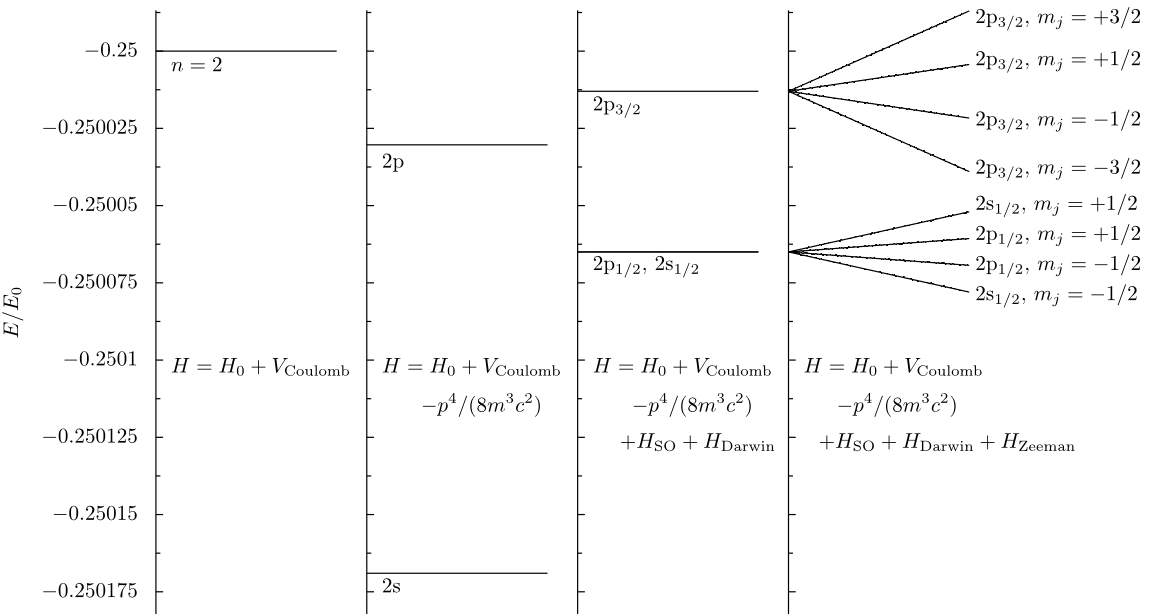
\includegraphics[width=1\linewidth]{src/n=2_hydrogen_fs.png}
    \caption{Fine-structure and Zeeman corrections for $n=2$}
    \label{fig:fs_zeeman}
\end{figure}
\begin{equation}
    E^1_{\mrm{so}}=\df{(E_n)^2}{mc^2}\cdot \df{n\left[j(j+1)-l(l+1)-3/4\right]}{l(l+1/2)(l+1)}
\end{equation}
Luckily, this combines neatly with the contribution from the 
relativistic correction to give the fine structure correction 
\begin{equation}
    E^1_{\mrm{fs}}=\df{(E_n)^2}{2mc^2}\left(3-\df{4n}{j+1/2}\right)
\end{equation}
\begin{table}[h!]
    \centering
    \begin{tabular}{|c|c|c|c|c|}
    \hline
    $n$ & $j$ & $l$ & $m_j$ & degeneracy \\ 
    \hline
    $1$ & $1/2$ & $\{0\}$ & $\{\pm 1/2\}$ & $2$ \\
    $2$ & $1/2$ & $\{0, 1\}$ & $\{\pm1/2\}$ & $4$ \\
        & $3/2$ & $\{1\}$    & $\{\pm1/2, \pm 3/2\}$ & $4$ \\
    $3$ & $1/2$ & $\{0\}$  & $\{\pm 1/2\}$ & $2$ \\
        & $3/2$ & $\{1, 2\}$ & $\{\pm 1/2, \pm3/2\}$ & $8$ \\
        & $5/2$ & $\{2\}$ & $\{\pm 1/2, \pm 3/2, \pm5/2\}$ & $6$ \\
    \hline
    \end{tabular}
    \caption{Energy levels of a spin $1/2$ particle for $n\leq 3$, arranged in $(n, j)$
    \label{tbl:hydrogen_fs}}
\end{table}
Combined with the Bohr formula, the energy now depend on both $n, j$. 
\begin{mdframed}
\begin{equation}\label{eqn:fs_energy_level}
    E_{nj} = -\df{(E_0)^2}{n^2}\left[1 + \df{\alpha^2}{n^2}\left(\df{n}{j+1/2} - \df 3 4\right)\right]
\end{equation}
\end{mdframed}
Our complete set of commuting observables are $H, L^2, S^2, J^2, J_z$ 
corresponding to quantum numbers $n, l, s, j, m_j$. 
Given $n$, we still have considerable degeneracy in $j, l, m_j$ (table~\ref{tbl:hydrogen_fs}).

\subsection{Zeeman effect}
Zeeman effect characterizes the energy corrections of an atom under external magnetic field. 
\begin{definition}[gyromagnetic ratio]
    The gyromagnetic ratio $\gamma$ of a system is the ratio between its magnetic moment and angular momentum. 
    \[ 
        \bm \mu = \gamma \mbf L
    \] 
    For a classically rotating body, $\gamma = \df q{2m}$. 
\end{definition}
\begin{definition}[Bohr magneton]
    The Bohr magneton provides the natural unit for gyromagnetic ratio of atomic systems. 
    \[ 
        \mu_B \equiv \df {e\hb}{2m_e}
    \] 
\end{definition}

For an electron, the gyromagnetic ratio for orbital motion and spin are different: that for the spin is roughly 
twice its classical value. Note that $\bm \mu$ scales inversely with mass. 
\begin{equation}
    \bm \mu = \bm \mu_l + \bm \mu_s = \df {\mu_B}{\hb}\left(\mbf L + 2\mbf S\right)
\end{equation}
In an external magnetic field $\mbf B$, a hydrogenic atom has the following correction 
\begin{equation}
    H'_Z = -\bm \mu \cdot \mbf B=\df {\mu_B} {\hb}\left(\mbf L + 2\mbf S\right)\cdot \mbf B
\end{equation}

\subsubsection{Weak-field Zeeman effect}

When $B\ll B_{\mrm{int}}$, we let $H^0=H_{\mrm{Bohr}}+H'_{fs}$. The zeroth-order eigenstates are given by 
by $L^2, S^2, J^2, J_z$. Without loss of generality, let $\mbf B = B\hat {\mbf z}$, then ($Z$ is for Zeeman)
\begin{equation}\label{eqn:zeeman_hamiltonian}
    H'_Z = \df{\mu_B B}{\hb}\left(L_z + 2S_z\right)
\end{equation}
After we have thus aligned the external field in the $z$-direction, 
the correction $H'_Z$ commutes with our complete set of 
operators and is diagonal in the $l, s, j, m_j$ basis, in which case 
\begin{equation}\begin{aligned}
    E^1_Z &= \df{\mu_B B}{\hb}\la L_z + 2S_z\ra \\ 
          &= \df{\mu_B B}{\hb}\left(J_z + \la S_z\right)\ra 
\end{aligned}\end{equation}
We now consider $\la S_z\ra$: the total angular momentum $\mbf J = \mbf L + \mbf S$ is constant, so the 
time average of $\mbf S$ is its projection along $\mbf J$ (see Griffiths for detailed explanation) 
\begin{equation}\begin{aligned}
    \la S_z\ra &= \df{\la \mbf{S\cdot J}\ra}{J^2}J_z \\ 
    &= \la \df 1 2\left(J^2 + S^2 - L^2\right)\ra\df{\hb m_j}{j(j+1)} \\
    &= \df{j(j+1)+s(s+1)-l(l+1)}{2j(j+1)}\hb m_j \\ 
    &= (g_J-1) m_j
\end{aligned}\end{equation}
Here we introduced the Landé $g$-factor $g_J$. The matrix element for energy correction is 
\begin{equation}
    \la n, l, s, j, m_j | H'_Z | n, l, s, j, m_j \ra = E^1_Z = \mu_B g_J m_j B
\end{equation}
Note that this correction is linear in $m_j$. 
Combined with equation~\ref{eqn:fs_energy_level}, the energy levels accounting for fine structure and 
weak-field Zeeman effect is 
\begin{equation}
    E_{nj} = -\df{(E_0)^2}{n^2}\left[1 + \df{\alpha^2}{n^2}\left(\df{n}{j+1/2} - \df 3 4\right)\right] + \mu_B g_Jm_j B
\end{equation}

\subsubsection{Strong-field Zeeman effect}
When the external magnetic field dominates the proton's magnetic field, we take $H^0=H_{\mrm{Bohr}}+H'_Z$ and 
$H'_{\mrm{fs}}$ to be the perturbation. 

Originally, $H_{\mrm{Bohr}}$ is degenerate in 
$l, s, m_l, m_s$, and equation~\ref{eqn:zeeman_hamiltonian} suggests that the 
states with the same $m_l+2m_s$ are degenerate eigenstates of $H^0$. 
To apply non-degenerate perturbation theory, 
our basis must arise from a set commuting operators complementing $H^0, H'_{\mrm{fs}}$ 
which additionally lifts the degeneracy in $l, s, m_l+2m_s$. 
One such set is $L^2, S^2, J^2, J_z$. 
\begin{equation}
    E^1_{\mrm{fs}} = \la n, l, m_l, m_s | H'_r + H'_{\mrm{so}} | n, l, m_l, m_s\ra 
\end{equation}
Here $\la H'_r\ra$ commutes with the operators for our basis, so we can use equation~\ref{eqn:rel_corr}. 
For the spin-orbit term, $\la S_zL_z\ra = \hb^2m_lm_s$. Substitute the indeterminate quotient 
with $1$ when $l=0$.
\begin{equation}
    E^1_{\mrm{fs}} = -\df{E_0}{n^3}\alpha^2 \left[\df 3 {4n} - \df{l(l+1) - m_lm_s}{l(l+1/2)(l+1)}\right]
\end{equation}

\begin{figure} % The [h!] tries to place the figure "here" as closely as possible
    \centering
    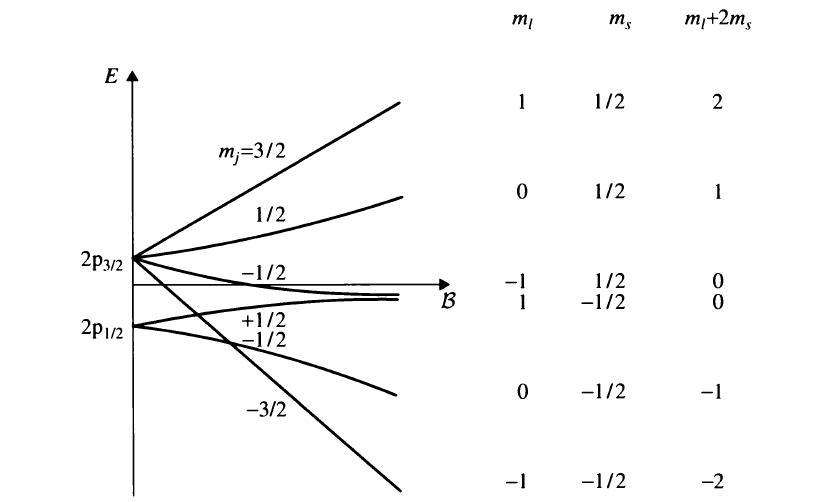
\includegraphics[width=1\linewidth]{src/zeeman.png}
    \caption{Zeeman effect for $n=2, l=1$}
    \label{fig:zeeman}
\end{figure}

Equation~\ref{eqn:zeeman_hamiltonian} dominates in the strong field regime,
while the fine structure characterized by~\ref{eqn:relativistic_hamiltonian}, 
\ref{eqn:spin_orbit_coupling} dominates in the weak field regime. 
The quantum numbers which distinguish between energy levels
in the strong-field regime is then $n, l, s, m_l+2m_s$, while those in the 
weak-field regime are $n, l, s, j, m_j$. The asymptotic slope in the figure above is 
determined by $m_l+2m_s$. 

\begin{figure}
    \centering
    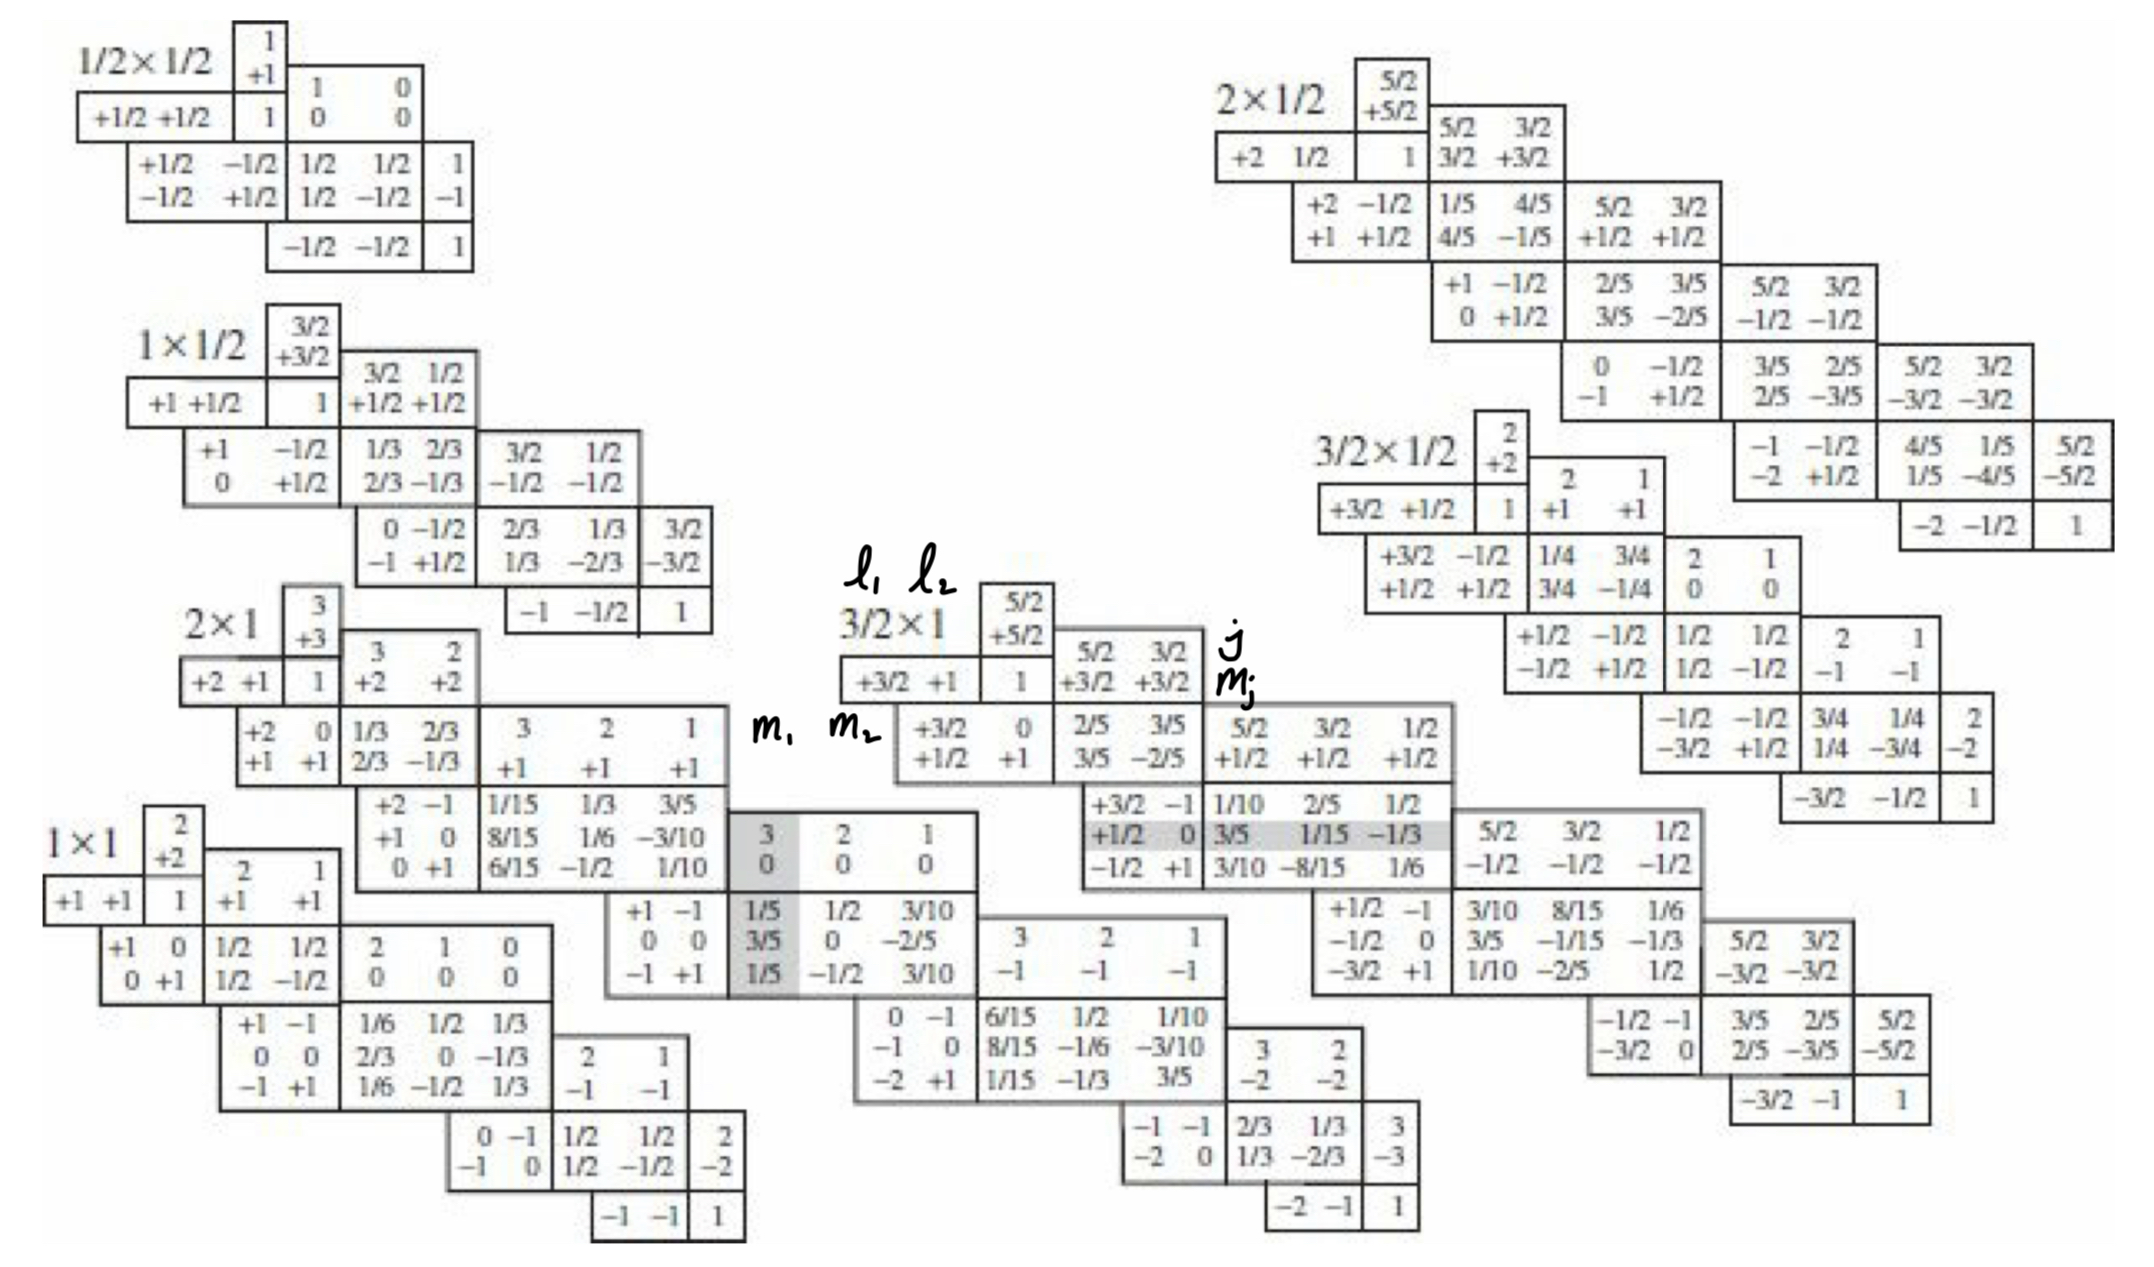
\includegraphics[width=1\linewidth]{src/clebsch-gordan.jpeg}
    \caption{Clebsch-Gordan coefficients}
    \label{fig:cg_coef}
\end{figure}

% \subsection{Hyperfine structure}
% The magnetic spin-dipole of a proton and electron are, for $g_p\approx 5.59, g_e\approx 2.00$:
% \begin{equation}
%     \bm \mu_p = \df{g_p e}{2m_p}\mbf S_p\quad \bm \mu_e = \df{g_e e}{2m_e}\mbf S_e
% \end{equation}
% The proton's dipole sets up a magnetic field which interacts with the electron's dipole, 
% yielding the energy correction 
% \begin{equation}
%     E^1_{\mrm{hf}} = \df{\mu_0 g_p e^2}{8\pi m_pm_e}
%         \ang{\df{3(\mbf S_p\cdot \hat r)(\mbf S_e\cdot \hat r) - \mbf S_p \cdot \mbf S_e}{r^3}}
%          + \df{\mu_0 g_pe^2}{3m_pm_e}\ang{\mbf S_p\cdot \mbf S_e}|\psi(0)|^2
% \end{equation}
% When $l=0$, the first term vanishes, leaving spin-spin coupling via 
% \begin{equation}\begin{aligned}
%     E^1_{\mrm{hf}} 
%     &= \df{\mu_0 g_pe^2}{3m_pm_e}|\psi(0)|^2 \ang{\mbf S_p\cdot \mbf S_e} \\ 
%     &= \df{\mu_0 g_pe^2}{6m_pm_e}|\psi(0)|^2 \ang{F^2 - S_e^2 - S_p^2}
% \end{aligned}\end{equation}
% Recalling equation~\ref{eqn:spin_orbit_coupling}. 
% The basis we have been using, using $I$ to denote 
% the nuclear spin, is $n, l, s, I, m_l, m_s, m_I$ corresponding to $L^2, S_e^2, S_p^2, L_z, S_{e, z}, S_{p, z}$. 
% the diagonal basis is in terms of the total spin $\mbf F =\mbf S_e + \mbf S_p $, given by 
% $L^2, S_e^2, S_p^2, F^2, F_z$ corresponding to $n, l, s, I, f, m_f$.

% \subsection{Stark effect}
% In the presence of an electric field with large wavelength compared to the 
% size of the atom, the first-order energy correction reads 
% \begin{equation}\begin{aligned}
%     H_{\mrm{Stark}} &= -\mbf{d\cdot E} = e\, \mbf{r\cdot E} \\ 
% \end{aligned}\end{equation}
% We take the original Hamiltonian $H_0 = H_\mrm{Bohr}+H_\mrm{fs}$. 
\section{Time-dependent Systems}

Consider quantum systems whose Hamiltonian may be time-dependent. 
For most systems, the Hamiltonian consists of a solvable time-independent $H^0$ and 
a time-dependent $H'(t)$. 
\[ 
    H(t)=H^0+H'(t)
\] 
When $H'(t)$ is weak compared to $H^0$, we may resort to 
time-dependent perturbation theory. 
Consider $H^0$ with eigenstates $\psi_a, \psi_b$ and energy $E_a, E_b$. 
For an arbitrary state, 
\[ 
    |\psi\ra = \sum c_n|n\ra 
\] 
The time-evolution of a state under $H^0+H'(t)$ is 
\begin{equation}\label{eqn:time-dependent solution}
    |\psi(t)\ra = \sum c_n(t) \exp\left(-\df i \hb E_n t\right) |n\ra 
\end{equation}
In general, $c_n(t)$ are time-dependent and only constantly $1$ when $\pd t H'(t) = 0$. 
The probability of finding state in $|n\ra$ at time $t$ is $|c_n(t)|^2$, 
which are subject to normalization 
\[ 
    \sum |c_n(t)|^2 = 1
\] 
Consider the Schrödinger equation for this system 
\begin{equation}\label{eqn:time-dependent Schrodinger}
    \pd t |\psi(t)\ra = -\df i \hb \left[H^0+H'(t)\right] |\psi(t)\ra
\end{equation}
Substituting equation~\ref{eqn:time-dependent solution} yields 
\[ \begin{aligned}
    i \hb \pd t \left[\sum c_n(t) \exp\left(-\df i \hb E_n t\right) |n\ra \right] &= 
        \left[H^0 + H'(t)\right]\left[\sum c_n(t) \exp\left(-\df i \hb E_n t\right) |n\ra \right] \\ 
\end{aligned}\] 
Expanding the left hand side (we suppress summation to avoid clutter) 
\[ 
    i \hb \pd t \left[c_n(t) \exp\left(-\df i \hb E_n t\right) |n\ra \right] =
    i\hb \dot c_n \exp\left(-\df i \hb E_nt\right)|n\ra 
        + E_n c_n \exp\left(-\df i \hb E_nt\right)|n\ra
\] 
On the right hand side, the first term cancels with the last term on the left hand side above 
\[ 
    H^0\left[c_n(t) \exp\left(-\df i \hb E_n t\right) |n\ra \right] 
        = E_n c_n \exp\left(-\df i \hb E_nt\right)|n\ra
\] 
The equation we're left with cannot be directly isolated component-wise for $n$ 
because $H'(t)$ is not generally diagonal. 
\begin{equation}
    \sum_n H'(t)c_n(t)\exp\left(-\df i \hb E_nt\right)|n\ra = \sum_n i \hb \dot c_n \exp\left(-\df i \hb E_nt\right)|n\ra
\end{equation}
To isolate $\dot c_m$, apply $\la m|$ and denote the matrix element $H'_{mn}(t)=\ang{m|H'(t)|n}$. 
\[
    \sum_n H'_{mn} \exp\left(-\df i \hb E_nt\right) c_n = i\hb \dot c_m \exp\left(-\df i \hb E_mt\right)
\] 
Let $\omega_{nm} = (E_n - E_m)/\hb$, the Schrodinger equation~\ref{eqn:time-dependent Schrodinger} 
may be rewritten exactly as a system of $n$ coupled first-order differential equations
\begin{equation}\label{eqn:time-dependent systems}
    \dot c_n(t) = -\df i \hb \sum_m H'_{nm}(t) \exp\left(i \omega_{nm} t\right) c_m(t)
\end{equation}



\subsection{Interaction Picture}
The following section is adapted from these 
\href{https://ocw.mit.edu/courses/8-06-quantum-physics-iii-spring-2018/89ef6d5958ee59bae9a91345c3d8c8e4_MIT8_06S18ch4.pdf}
{lecture notes} from MIT. 
We may rephrase the derivation in the previous section more concisely 
in terms of the interaction picture. 
We adopt a frame in which the energy eigenstates of $H^0$, as they would normally evolve, 
remains constant. Formally, consider the transform 
\[\begin{aligned}
    |\tilde \psi(t)\ra &= U(t)^\dag|\psi(t)\ra , \quad U(t) &= \exp\left(-\df i \hb H^0 t\right)
\end{aligned}\] 
Note that $[H^0, U(t)] = 0$, the Schrodinger equation transforms accordingly. 
We use the subscript to denote time variable to reduce clutter: 
\leqalign{eqn:transformed se'}{
    \pd t |\tilde \psi_t\ra &= \pd t \left(U^\dag_t |\psi_t\ra \right)  
    = \df i \hb H^0 |\tilde \psi_t\ra + U^\dag_t \left(\pd t |\psi_t\ra \right) \\ 
    &= \df i \hb H^0 |\tilde \psi_t\ra - U^\dag_t \left[\df i \hb (H^0+H'_t)|\psi_t\ra \right] \\ 
    &= \df i \hb H^0|\tilde \psi_t\ra - \df i \hb \left(U_t^\dag H^0 U_t\right)\left(U_t^\dag |\psi_t\ra\right) 
        - \df i \hb \left(U_t^\dag H_t'U_t\right)\left(U_t^\dag |\psi_t\ra\right) \\ 
    &= -\df i \hb \left(U_t^\dag H_t'U_t \right) U_t^\dag |\psi_t\ra = -\df i \hb \tilde H_t' |\tilde \psi_t\ra
}
This frame change eliminates $H^0$ and leaves only $\tilde H'_t=U_t^\dag H_t'U_t$. 
Let $\{c_j(t)\}$ the expansion of the ket 
in our new frame with respect to the eigenbasis $|\psi_{n}\ra$ of $H^0$
\malign{
    |\tilde \psi_t\ra = \sum c_n(t) |\psi_{n}\ra 
}
These are exactly the de-wiggled coefficients we have introduced in the previous section. 
We can recover the evolution of the ket in our original frame by 
$|\psi_t\ra = U_t|\tilde \psi_t\ra$ by $U_t$, which 
is diagonal in this eigenbasis 
\[ 
    |\psi_t\ra = U_t \sum c_n(t)|\psi_n\ra  = \sum e^{-iE_nt/\hb} c_n(t)|\psi_n\ra 
\] 
In terms of this concrete basis, the Schrodinger equation~\ref{eqn:transformed se'} reads 
\[ 
    \dot {\tilde c}_n(t) = \la \psi_n| \left(\pd t |\tilde \psi_t\ra \right)
    = -\df i \hb \sum_m \tilde c_m(t) \la \psi_n|\tilde H'_t|\psi_m\ra 
\] 
We can simplify the matrix element by noting that 
\[ 
    \la \psi_n|\tilde H'_t|\psi_m\ra = \la \psi_n|e^{iH^0t/\hb}H'_te^{-iH^0t/\hb}|\psi_m\ra 
    = e^{i(E_n - E_m)t/\hb} H'_{nm}(t)
\] 
This leaves us equation~\ref{eqn:time-dependent systems}. 
\subsection{Time-Dependent Perturbation Theory}
So far everything is exact. To obtain a perturbative solution, introduce 
$\lambda$ and assume that $|\tilde \psi_t\ra$ can be expanded in $\lambda$:
\[\begin{aligned}
    H_t &= H^0 + \lambda H'_t \\ 
    |\tilde \psi_t\ra &= |\tilde \psi^0_t\ra + \lambda |\tilde \psi^1_t\ra + 
        \lambda^2|\tilde \psi^2_t\ra + \cdots \\ 
    \pd t |\tilde \psi_t\ra &= -\df i \hb \lambda \tilde H'_t|\tilde \psi_t\ra 
\end{aligned}\] 
Equating by powers of $\lambda$, the time-derivative of $n$-th component is coupled to 
$H'_t$ acting on $(n-1)$-th component. 
\begin{equation}\begin{aligned}\label{eqn:time-dependent perturbation}
    \pd t |\tilde \psi^0_t\ra &= 0 \\ 
    \pd t |\tilde \psi^1_t\ra &= -\df i \hb \tilde H'_t|\psi^0_t\ra \\ 
    \vdots \quad &= \quad \vdots \\ 
    \pd t |\tilde \psi^{n+1}_t\ra &= -\df i \hb \tilde H'_t|\psi^n_t\ra 
\end{aligned}\end{equation}
Our interacting picture transform degenerates to the identity at $t=0$. 
Equating the power series approximation, which holds for all $\lambda$, 
yields the initial conditions 
\begin{equation}\begin{aligned}
    |\psi_0\ra &= |\tilde \psi^0_0\ra + \lambda |\tilde \psi^1_0\ra + \cdots \\ 
    |\tilde \psi^0_0\ra &= |\tilde \psi_t^0\ra = |\psi_0\ra \\ 
    |\tilde \psi^n_\sim\ra &= 0, \quad n>0
\end{aligned}\end{equation}
An initial state $|\psi_0\ra$ gives us the constant $(n=0)$-th order solutions $|\tilde \psi^0_t\ra$. 
in the transformed frame, $|\tilde \psi_0\ra$ is constant, i.e. the zeroth order 
solution evolves only according to $H^0$. 
Using the zero initial condition, 
The following terms in equation~\ref{eqn:time-dependent perturbation} is solved by 
succesive integration. 
\begin{equation}\begin{aligned}
    |\tilde \psi_t^1\ra &= -\df i \hb \int_0^t H'_{t'} |\psi_{t'}^0\ra \, dt' \\ 
    |\tilde \psi_t^2\ra &= -\df i \hb \int_0^t H'_{t'} |\psi_{t'}^1\ra \, dt'
    = -\df i \hb \int_0^t H'_{t'} \left(-\df i \hb \int_0^{t'} H'_{t''} |\psi_{t''}^0\ra \, dt''\right) \, dt' \\ 
    &= -\df 1 {\hb^2}\int_0^t H'_{t'}\int_0^{t'} H'_{t''} |\psi_{t''}^0\ra \, dt''\, dt' \\ 
    |\tilde \psi_t^3\ra &= -\df i \hb \int_0^t H'_{t'}|\psi_{t'}^2\ra\, dt' = \cdots 
\end{aligned}\end{equation}
In concrete terms, consider an initial state $|\psi_0\ra$. 
We first consider the Fourier expansion of a ket $|\tilde \psi_t\ra$ in the 
transformed frame in terms of the eigenstates of $H^0$. 
\[ 
    |\tilde \psi_t\ra = \sum_k |\tilde \psi_t^k\ra = \sum_{k, j} \tilde c_j^k(t) |j\ra 
\] 
They are related to the Fourier expansion of $|\psi_t\ra$ in the original frame via 
\[ 
    \tilde c_j^k(t) = \exp\left(-\df i \hb E_j t\right)c_j^k(t)
\] 
In concrete components, the zeroth order correction is the constant initial condition. 
\[\begin{aligned}
    |\tilde \psi^0_t\ra &= \sum \tilde c_j^0(t) |j\ra = \sum \exp\left(-\df i \hb E_j t\right) c_j^0 |j\ra \\ 
    |\psi_t^0\ra &= \exp\left(\df i \hb H^0 t\right)|\tilde \psi_0\ra = |\psi_0\ra 
\end{aligned}\] 
Introduce $\omega_{kj} = \exp(i(E_k-E_j)/\hb)$, the first-order components read 
\[\begin{aligned}
    \tilde c_k^1(t)
    &= \la k|\tilde \psi_t^1\ra 
        = -\df i \hb \la k |\int_0^t H'_{t'}  \sum \exp\left(-\df i \hb E_j t\right) c_j^0 |j\ra \, dt' \\ 
        &= -\df i \hb \sum_j \int_0^t \la k|H'_{t'}|j\ra \exp\left(-\df i \hb E_j t\right) c_j^0\, dt' \\ 
    c_k^1 &= -\exp\left(\df i \hb E_k t \right) \tilde c_k^1(t) \\
    &= -\exp\left(\df i \hb E_k t \right)\df i \hb \sum_j \int_0^t \la k|H'_{t'}|j\ra \exp\left(-\df i \hb E_j t\right) c_j^0\, dt' \\ 
    &= -\df i \hb \sum_j c_j(0) \int_0^t \la k|H'_{t'}|j\ra \exp(i\omega_{kj})\, dt'
\end{aligned}\] 
The second-order components read 
\[\begin{aligned}
    \tilde c_k^2(t)
    &= \la k|\tilde \psi_t^2\ra = -\df 1 {\hb^2}\int_0^t \la k| H'_{t'}\int_0^{t'} H'_{t''} |\psi_{t''}^0\ra \, dt''\, dt'\\ 
    &= -\df 1 {\hb^2}\sum_j \int_0^t \la k| H'_{t'}|j\ra \int_0^{t'} \la j|H'_{t''} |\psi_{t''}^0\ra \, dt''\, dt'\\ 
    &= -\df 1 {\hb^2}\sum_{j, l} \int_0^t \la k| H'_{t'}|j\ra \int_0^{t'} \la j|H'_{t''} \exp\left(-\df i \hb E_l t\right) c_l^0|l\ra  \, dt''\, dt'\\ 
    c_k^2(t) &= -\exp\left(\df i \hb E_k t \right) \tilde c_k^2(t) \\
    &= -\df 1 {\hb^2}\sum_{j, l} \int_0^t \exp\left(\df i \hb (E_k-E_j+E_j) t \right) \la k| H'_{t'}|j\ra \int_0^{t'} 
        \exp\la j|H'_{t''} \exp\left(-\df i \hb E_l t\right) c_l^0|l\ra  \, dt''\, dt'\\ 
    &= -\df 1 {\hb^2}\sum_{j, l} c_l(0) \int_0^t \exp(i\omega_{kj}t)\la k| H'_{t'}|j\ra \int_0^{t'} \exp(i\omega_{jl}t)\la j|H'_{t''} |l\ra  \, dt''\, dt'\\ 
\end{aligned}\] 
Taken together and let $H'_{ab}(t) = \la a|H'(t)|b\ra$, the second-order approximation is 
\leqalign{eqn:sec_order_time_perturbation}{
    c_k(0) &-\df i \hb \sum_j c_j(0) \int_0^t H'_{kj}(t') \exp(i\omega_{kj}t)\, dt' \\ 
    &-\df 1 {\hb^2}\sum_{j, l} c_l(0) \int_0^t \exp(i\omega_{kj}t) H'_{kj}(t') \int_0^{t'} \exp(i\omega_{jl}t)H'_{jl}(t'')\, dt''\, dt'
}
Griffiths forgoes the polynomial picture altogether. 
Substitute $c_m(t)=c_m(0)$ into 
the right hand side of equation~\ref{eqn:time-dependent systems} to obtain 
the first order coefficients (not corrections)
\begin{equation}\label{eqn:first-order coefficient}
    c_n^{(1)}(t) = c_n(0) - \df i \hb \sum_m c_m(0)\int_0^t H'_{nm}(t')\exp(i\omega_{nm}t')\, dt'
\end{equation}
For the second-order, 
substitute $c_m(t)$ in equation~\ref{eqn:first-order coefficient} into~\ref{eqn:time-dependent systems}. 

We wish to emphasize the theme of polynomial approximation in perturbation theory, 
even in time-dependent systems. 
We start by introducing a tilde frame which eliminates $H^0$ and 
assuming that time-evolution in this frame is expandable in succesive powers of $\lambda$. 
In this frame, the zeroth order solution is constant, and higher-order corrections are coupled 
to the perturbative action of $H'$ on the immediately lower order. We switch back to the original 
frame after performing the polynomial approximation. 


\subsection{Sinusoidal Perturbations}
Consider a two-level system with sinusoidal perturbation 
\leqalign{eqn:sinusoidal_perturb}{
    H'(r, t) &= V(r)\cos \omega t \\ 
    H'_{ab}(t) &= \la \psi_a | V |\psi_b\ra \cos\omega t = V_{ab}\cos \omega t
}
Assuming initial level $a$ and that diagonal matrix elements vanish, to 
the first order in \ref{eqn:sec_order_time_perturbation}
\[\begin{aligned}
    c_b(t) 
    &= -\df i \hb V_{ba}\int_0^t \cos\omega t \exp(i\omega_{ba}t)\, dt'\\ 
    &= -\df {i V_{ba}}{2\hb} \int_0^t \left[\exp(i(\omega_0 + \omega) t') + \exp(i(\omega_0 - \omega)t')\right]\, dt' \\ 
    &= -\df {V_{ba}}{2\hb}\left[\df{\exp(i(\omega_0 + \omega)t) - 1}{\omega_0 + \omega} + \df{\exp(i(\omega_0 - \omega)t) - 1}{\omega_0 - \omega}\right]
\end{aligned}\] 
Far-detuned frequency have negligible transition rates. Assuming $\omega_0 + \omega \gg |\omega_0 - \omega|$. 
Drop the first term. Let $\Delta_\omega = \omega_0 - \omega$ 
\malign{
    c_b(t) 
    &\approx -\df {V_{ba}}{2\hb} \df{\exp(i\Delta_\omega t/2)}{\Delta_\omega }
        \left[\exp(i\Delta_\omega t/2) - \exp(-i\Delta_\omega t/2)\right] \\ 
    &= -i\df {V_{ba}}{\hb} \df{\sin\left(\Delta_\omega t/2\right)}{\Delta_\omega } e^{i\Delta_\omega t/2}
}
The following transition probability should be trusted for $\omega_0 + \omega \gg |\omega_0 - \omega|$ and 
relatively small probability. The most significant feature is flopping. 
\leqalign{eqn:flopping}{
    P_{a\to b}(t)\approx \df{|V_{ab}|^2}{\hb^2} 
        \df{\sin^2\left(\Delta_\omega t/2\right)}{\Delta_\omega^2}
}
\subsection{Rabi Flopping}
Sinusoidal perturbation may be solved exactly if we begin by approximating 
\[ 
    H'(r, t) = V(r)\cos(\omega t) \to \df V 2 e^{-i\omega t}
\] 
Here, we ignore the $e^{i\omega t}$ earlier: in the Hamiltonian instead of as a perturbed term. 
The perturbation under this approximation is not Hermitian, but it allows us to solve 
equation~\ref{eqn:time-dependent systems}. 
Again, consider a two-level system with 
$\omega_0 = (E_b - E_a)/\hb>0$ starting out in state $a$, then 
\[
    \dot c_a(t) = -\df i \hb H'_{ab}(t)e^{-i\omega_0 t} c_b(t)
    ,\quad \dot c_b(t) = -\df i \hb H'_{ba}(t)e^{i\omega_0 t}c_a(t)
\] 
We assume again that diagonal matrix elements vanish. 
Take another derivative of the equations above to uncouple $c_a, c_b$. 

\subsection{Interaction with EM waves}
% Consider an EM wave incident on a hydrogenic atom: 
% \[\begin{aligned}
%     H &= \df 1 {2m}\left(-i\hb \nabla - qA\right)^2 + \Phi q + V_{\mrm{Coulomb}}(r)  \\ 
%         &= \df 1 {2m}\left(p - qA\right)^2 + \Phi q + V_{\mrm{Coulomb}}(r) 
% \end{aligned}\] 
% Choose the Coulomb gauge 
% \[\begin{aligned}
%     \nabla\cdot A &= 0 \\ 
%     \Phi(r, t) &= 0
% \end{aligned}\] 
% Recall the electric component of constant-polarization monochromatic light propagating in 
% direction $k$ with polarization along $E_0$: 
% \[ 
%     E(r, t) = E_0 e^{i(k\cdot r - \omega t)}
% \] 
% For a (constant-polarization) plane wave with polarization along $A_0$ propagating along $r$
% \[ 
%     A = \mrm{Re}\left[A_0 \, e^{i(k\cdot r - \omega t)}\right]
% \] 
% Now $k\cdot E_0 = 0$. Also recall that 
% \[ 
%     E = -\nabla \Phi - \pd t A
% \] 
% Under the Coulomb gauge, $E_0\|A_0$. In particular, $E_0 = \df \omega 2 A_0 i$. 

% For the Coulomb gauge, $[A, p] = 2 A p$, expand out the Hamiltonian to obtain 

% The Hamiltonian expands to (recall that we're focused on the reals!)
% \[ 
%  H = \left(\df {p^2}{2m} + V(r)\right) +
%      \df e {2m} \left[e^{i(k\cdot r - \omega t)}A_0
%         + e^{-i(k\cdot r - \omega t)}\bar A_0\right] p 
% \] 
% Let $a$ denote the full set of quantum numbers $n, l, m, m_s$. 

% We wish to consider how a plane wave interacts with an electron in 
% a special state $a$. Consider $c_b(t), b\neq a$. According to the perturbation equation 
% and our initial conditions,
% \[ 
%     c_b(t) = - \df i \hb c_a(i)\int_0^t dt' H'_{ba}(t') \exp(i\omega_{ba}t')
% \] 
% We first compute the matrix element. Recall the expanded Hamiltonian 
% \[\begin{aligned}
%     H'_{ba}(t) 
%     &= \ang{b|H'(t)|a} \\ 
%     &= \int d^3r\, \psi^*_b(r)H'_t(r)\psi_a(r) \\ 
%     &= \df e {2m}\int d^3r\, \psi^*_b(r) \left[e^{i(k\cdot r - \omega t)}A_0
%         + e^{-i(k\cdot r - \omega t)}\bar A_0\right] p\, \psi_a(r)
% \end{aligned}\] 
% In the limit $\lambda \gg a_B$, the electromagnetic wave is locally constant. Recall 
% that $k = 2\pi / \lambda$. We can expand $e^{i(k\cdot r - \omega t)}$ in terms of $r$ and 
% only take the first order. 
% \[ 
%     e^{ik\cdot r} = 1
% \] 
% The integral simplifies to 
% \[\begin{aligned}
%     H'_{ba}(t) 
%     &= \df e {2m}\int d^3r\, \psi^*_b(r) \left[e^{- i\omega t}A_0
%         + e^{i \omega t}\bar A_0\right] p\, \psi_a(r)
% \end{aligned}\] 
% Now, to help us compute the integral \textbf{(prove this!!)}
% \[ 
%     \left[r, \df{p^2}{2m}\right] = \df 1 {2m} \sum\left([r_i, p_i]p_i + p_i[r_i, p_i]\right) = \df{i\hb}{m}p
% \] 
% Replace $p=\df m {i\hb} [r, H_0]$ into the equation above 
% \[ \begin{aligned}
%     H'_{ba}(t) 
%     &= \df{e}{2i\hb}\int d^3 r \psi_b^*(r)
%         \left[\exp^{-i\omega_{ba}t}A_0 r (E_a - E_b) + c.c\right]\psi_a(r)  \\ 
%     &= \df{i\omega_{ba}}{2}A_0 \la b |e\, r|a\ra \left[\exp(-i\omega_{ba}t) + \exp(i\omega_{ba}t)\right] \\ 
%     &= i\omega_{ba}A_0 \ang{b|e\, r|a}\mrm{Re}\left(e^{i\omega_{ba}t} + e^{-i\omega_{ba}t}\right)
% \end{aligned}\] 
Consider a monochromatic electromagnetic wave incident upon a hydrogenic atom. 
When its wavelength is long compared to the Bohr radius, to the first order of this ratio, 
the atom effectively acts as a dipole within a sinusoidally oscillating electric field: 
\[ 
    H' = -q E_0 z\cos \omega t
\] 
Then the matrix element for the perturbation reads 
\[ 
    H'_{ba}(t) = -q\la \psi_b|z|\psi_a\ra E_0\cos \omega t
\] 


\subsubsection{Absorption, Stimulated Emission}
The selection rule for spatial 
components dictate $\Delta l = \pm 1$, so diagonal matrix elements for $H'$ always vanish.
Equivalently, note that 
$z|\psi|^2$ is odd in $z$. Then the problem is as in~\ref{eqn:sinusoidal_perturb} with 
$V_{ba}=-q\la \psi_b|z|\psi_a\ra E_0$. Substitution into equation~\ref{eqn:flopping} yields 
\leqalign{eqn:monochromatic transition}{
    P_{a\to b}(t) = P_{b\to a}(t) = 
    \left(\df{q\la \psi_a|z|\psi_b\ra E_0}{\hb}\right)^2
        \df{\sin^2\left(\Delta_\omega t/2\right)}{\Delta_\omega^2}
}
Equal absorption and stimulation probability is by 
the first-order formula~\ref{eqn:first-order coefficient}: 
\[ 
    H'_{nm} = \overline{H'_{mn}}, \quad \omega_{nm} = -\omega_{mn}
\] 
The transition probability $P_{a\to b}(t) = |c_b(t)|^2$, computed with 
initial conditions $c_n(0) = \delta_{na}$. 


\subsubsection{Spontaneous Emission}
We first generalize the perturbation result from a monochromatic, polarized, 
single-frequency electromagnetic wave to the general case. 
Recall the energy density of electromagnetic wave
\[
    u = \df {\epsilon_0}{2}E_0^2
\]
Substitute $E_0$ with this equation into equation~\ref{eqn:monochromatic transition} 
yields, for $V_{ab} = q\la \psi_a|z|\psi_b\ra$ 
\[ 
    P_{b\to a}(t) = \df{2u|V_{ab}|^2}{\epsilon_0 \hb^2} \cdot 
        \df{\sin^2\left(\Delta_\omega t/2\right)}{\Delta_\omega^2}
\] 
Let $du=\rho(\omega)\, d\omega$ denote some distribution of energy-frequency density. 
When the different components are phase-decorrelated (incoherent), we 
can conveniently perform the integral over the probability instead of the amplitude, yielding 
\[ 
    P_{b\to a}(t) = \df{2|V_{ab}|^2}{\epsilon_0 \hb^2} 
        \int_0^\infty d\omega\, \rho(\omega)\left[\df{\sin^2\left(\Delta_\omega t/2\right)}{\Delta_\omega^2}\right]
\] 
The bracket term is sharply peaked about $\omega = \omega_0$. 
We pull $\rho(\omega)$ outside the integral 
\[ 
    P_{b\to a}(t) \approx \df{2|V_{ab}|^2}{\epsilon_0 \hb^2} \rho(\omega_0)
    \int_0^\infty d\omega\, \left[\df{\sin^2\left(\Delta_\omega t/2\right)}{\Delta_\omega^2}\right]
    =\df{\pi |V_{ab}|^2}{\epsilon_0 \hb^2}\rho(\omega_0)t
\] 
Note that integrating over an incoherent frequency spectrum gets rid of the flopping. 
\begin{definition}[transition rate]
    The transition rate between two levels is defined as 
    \[ 
        R_{b\to a} = \pd t P_{b\to a}
    \] 
\end{definition}
The transition rate between two levels in an incoherent spectrum $\rho(\omega)$ with 
uniform polarization and direction is 
\[ 
    R_{b\to a} = \df{\pi}{\epsilon_0\hb^2}|V_{ab}|^2 \rho(\omega_0)
\] 
Averaging over all propagation and polarization directions introduces a 
factor of $1/3$ and $z\mapsto \mbf r$ since we are not restricted to the $z$ direction. 
\begin{mdframed}
\[ 
    R_{b\to a} = \df{\pi}{3\epsilon_0\hb^2}q^2|\la \psi_a|\mbf r|\psi_b\ra|^2 \rho(\omega_0) 
    = B\rho(\omega_0),\quad\quad B = \df{\pi q^2|\la \psi_b|\mbf r|\psi_a\ra|^2}{3\epsilon_0\hb^2}
\] 
\end{mdframed}
Denote by $A$ the rate of particles leaving the higher energy level $B$ by spontaneous emission. 
\malign{
    d_t N_b 
        &= -N_bA - N_b R_{b\to a} + N_a R_{a\to b} \\ 
        &= -N_bA - N_b B \rho(\omega_0) + N_a B \rho(\omega_0) \\ 
}
In thermal equilibrium $d_tN_b=0$, $N_a/N_b = \exp(\hb \omega_0 / k_B T)$. 
Planck radiation formula gives 
\[ 
    \rho(\omega_0) = \df A {(N_a/N_b - 1)B} = \df A {(e^{\hb \omega_0 / \tau} - 1)B} 
        = \df{\hb \omega_0^3}{\pi^2c^3(e^{\hb\omega / \tau} - 1)}
\] 
This gives us the spontaneous emission coefficient 
\begin{mdframed}
\[ 
    A = \df{\omega_0^3q^2|\la \psi_b|\mbf r|\psi_a\ra|^2}{3\pi \epsilon_0 \hb c^3}
\] 
\end{mdframed}
Assuming only spontaneous emission along decay modes with rate coefficients
$A_1, A_2, \cdots$ and no replenishing mechanism, the population obeys 
\[ 
    dN = -\left(\sum A_n\right) N\, dt \implies N(t) = N(0)\exp\left(-\df t \tau\right),
    \quad \tau = \left(\sum A_n\right)^{-1}
\] 
Here $\tau$ is the state's lifetime.
Recall the selection rules: matrix elements for a vector $\mbf r$ obeys 
\begin{mdframed}
\[\begin{aligned}
    \Delta l = \pm 1,&\quad\quad \Delta m = 0, \pm 1, \quad \text{for any component} \\ 
    \Delta m = 0 \implies \la n'l'm|x|nlm\ra &= \la n'l'm|y|nlm\ra = 0 \\ 
    m' = m\pm 1 \implies \la n'l'm'|x|nlm\ra &= \pm i \la n'l'm|y|nlm\ra = 0, 
    \la n'l'm'|z|nlm\ra = 0
\end{aligned}\]
\end{mdframed}
These rules (Griffiths 11.76) are very handy when evaluating transitions rates. 

\subsection{Bound to Continuum Transitions}
We can discretize a continuous energy spectrum by confining the system in a box of size 
$L$, use periodic (or impenetratable, the former is usually more convenient) boundary conditions 
to obtain a discrete spectrum, then take the limit as $L\to \infty$. This gives us the 
state density $\rho(E)$ with respect to energy. 
We consider a system, under sinusoidal perturbation, 
transitioning from a bound state to a continuum state 
with an energy in finite range $\Delta E$ about $E_f$. 
Integrating equation~\ref{eqn:flopping} yields 
\[ 
    P_{a\to (E_b, \Delta E)}(t) = 
    \int_{E_b - \Delta E / 2}^{E_b + \Delta E/2} \df{|V_{ab}|^2}{\hb^2} 
    \left[\df{\sin^2((\omega_0 - \omega) t/2)}{(\omega_0 - \omega)^2}\right]\rho(E)\, dE 
\] 
Here $\omega_0(E) = (E - E_a)/\hb$, and $\rho(E)\, dE$ is the number of states of between $E, E+dE$. 
The bracket quantity is sharply peaked about $E=E_f$ with width $4\pi \hb/t$. For $t\gg 1$, 
approximate by pulling $\rho(E)$ out of the integral, which we also extend to infinity 
\[ 
    P_{a\to E_b}(t\to \infty) = \df \pi {2\hb} |V_{ab}|^2 \rho(E_b)t 
\] 
The transition rate in this limit is known as Fermi's Golden Rule (sinusoidal perturbations)
\begin{mdframed}\leqalign{eqn:fermi's golden rule}{
    R_{a\to b} = \df \pi {2\hb} |V_{ab}|^2 \rho(E_b)
}\end{mdframed}
Recall that $H'(r, t)=V(r)\cos(\omega t)$ and $V_{ab}=\la \psi_a|V(r)|\psi_b\ra$. 

\subsection{Adiabatic theorem}
The reference for this section is Weinberg, \textit{Lectures on Quantum Mechanics, VI.6}. 

We consider a parameterized family of Hamiltonians $H_s$, where $s$ is a slowly varying 
function $s(t)$ of time. By Hermiticity, $H_s$ is diagonalizable for every $s$. 
Given a smooth path $s$ with subscript $0$ denote the initial condition $t=0$, 
we can track how the eigenbasis $\{|n_s\}$ of $H_s$ smoothly varies with $s(t)$ 
via a parameterized unitary $U(s)$ such that 
\[ 
    |n_s\ra = U(s)|n_0\ra \implies U_s = \sum_n |n_s\ra\la n_0|,\quad U(s_0) = \mrm{Id}
\] 
Consider a frame change parameterized by $U(t)$ 
\[ 
    \tilde H_s = U_s^\dag H_s U_s 
\] 
In this frame, the eigenvectors of $\tilde H_s$ are constant. Only eigenvalue 
dependence on $s$ remains 
\[ 
    \tilde H_s |n_0\ra = U_s^\dag H_s |n_s\ra = E_n(s) U_s^\dag|n_s\ra = E_n(s)|n_0\ra 
\] 
Consider the corresponding state transformation (we now suppress $|n_0\ra = |n\ra$)
\[ 
    |\tilde \psi(t)\ra = U_s^\dag |\psi(t)\ra 
\] 
The Schrödinger equation transforms as 
\malign{
    \pd t |\tilde \psi(t)\ra 
    &= \left(\pd t U_{s(t)}^\dag\right)|\psi(t)\ra + 
        U^\dag_s \left(\pd t |\psi(t)\ra \right) \\ 
    &= \left(\pd t U_{s(t)}^\dag\right)|\psi(t)\ra + 
        U^\dag_s \left(-\df i \hb H_s |\psi(t)\right) \\
    &= \left(\pd t U_{s(t)}^\dag\right)U_s |\tilde \psi(t)\ra 
        -\df i \hb \tilde H_s |\tilde \psi(t)\ra \\ 
    &= -\df i \hb \left[\tilde H_{s(t)} + \Delta(t)\right]|\tilde \psi(t)\ra 
}
This looks like the ``normal'' time-evolution of the frame-shifted state 
under the frame-shifted Hamiltonian, with an additional term 
\[ 
    \Delta(t) = i\hb \left(\pd t U_{s(t)}\right)^\dag U_s
\] 
We introduce another coordinate transform parameterized by the 
unitary operator $V(t)$ well-defined by the following differential equation, for $-i\tilde H_{s(t)}$ 
correctly skew-Hermitian: 
\[ 
    \pd t V(t) = -\df i \hb \tilde H_{s(t)}V(t)
\] 
In the eigenbasis $\{|n_0\ra\}$ for $\tilde H_{s(t)}$ (and also for $H_{s(0)}$) 
the solution is explicit.  
\[ 
    \la n|V(t)|m\ra = \delta_{nm}\exp \left(-\df i \hb\int_0^t E_n(s(t'))\, dt' \right)
    = \delta_{nm} \exp\left(i\phi_n(t)\right)
\] 
Here $\phi_n(t)$ is called the dynamical phse 
\[ 
    \phi_n(t) = -\df 1 \hb \int_0^t E_n(s(t'))\, dt'
\] 
This frame further eliminates dependence on $\tilde H_{s(t)}$. Define the transforms 
\malign{
    |\bar \psi_t\ra = V(t)^\dag |\tilde \psi(t)\ra &=  V(t)^\dag U_s^\dag |\psi(t)\ra  \\ 
    \bar \Delta(t) &= V(t)^\dag \Delta(t) V(t)
}
$\tilde H_{s(t)}$ and $V(t)$ shares an eigenbasis.  
Only $\bar \Delta(t)$ remains in the Schrödinger equation: 
\malign{
    \pd t |\bar \psi(t)\ra 
    &= \left(\pd t V(t)^\dag \right)|\tilde \psi(t)\ra + V(t)^\dag \pd t |\tilde \psi(t)\ra \\ 
    &= \df i \hb \tilde H_{s(t)}V(t)^\dag |\tilde \psi(t)\ra 
        -\df i \hb V(t)^\dag  \left[\tilde H_{s(t)} + \Delta(t)\right]|\tilde \psi(t)\ra  \\ 
    &= -\df i \hb V(t)^\dag \Delta(t)|\tilde \psi(t)\ra = -\df i \hb \bar \Delta(t)|\bar \psi(t)\ra 
}
Consider the matrix elements of $\overline \Delta_{nm}(t)$ under its eigenbasis $\{|n\ra\}$
\malign{
    \la n|\bar \Delta(t)|m\ra &= \la n|V(t)^\dag \Delta(t)V(t)|m\ra = 
    \exp\left(i[\phi_m(t)-\phi_n(t)]\right) \la n|\Delta(t)|m\ra  \\ 
    &= \la n|\Delta(t)|m\ra \exp \left[\df i \hb \int_0^t dt'\, E_n(s(t')) - E_m(s(t'))\right]
} 
In the absence of degeneracy, when the rate of change of $s(t)$ is very small compared 
to $|E_n(s) - E_m(s)|/\hb$, any duration that is significant with respect to $\Delta s(t)$ 
will cause the phase factor to oscillate many times. The only components of $\bar \Delta(t)$ 
which consistently contribute are the diagonal elements, by which 
\malign{
    \bar \Delta(t) 
    &= \sum_n \la n|\bar \Delta(t)|n\ra \, |n\ra \la n| 
    = \sum_n \la n| \Delta(t)|n\ra \, |n\ra \la n| \\ 
    &= \sum_n \la n | \left[i\hb \left(\pd t U_{s(t)}\right)^\dag U_s\right] |n\ra \, |n\ra \la n| \\ 
    &= i\hb \sum_n \left(\pd t \la n_s|\right)|n_s\ra \, |n\ra \la n| \\ 
    &= \sum \rho_n(t)|n\ra \la n|, \quad \rho_n(t) = i\hb \left(\pd t \la n_s|\right)|n_s\ra 
}
The Schrodinger equation in the bar frame solves to 
\malign{
    |\bar \psi(t)\ra 
    &= \sum_n \exp(i\gamma_n(t)) \la n|\bar \psi_0\ra |n\ra 
    = \sum_n \exp(i\gamma_n(t)) \la n|\psi_0\ra |n\ra 
}
In particular, note that $|\bar \psi(0)\ra = |\psi(0)\ra$ since both transforms 
are trivial at $t=0$. Here $\gamma_n(t)$ denotes the Berry phase 
\[ 
    \gamma_n(t) = -\df 1 \hb \int_0^t \rho_n(t')\, dt'
\] 
Change back to the original frame, here $V(t)$ introduces $\phi_n(t)$ and 
$U_s$ effects $|n\ra \mapsto |n_s\ra$. 
\malign{
    |\psi(t)\ra 
    &= U_{s(t)}V(t)|\bar \psi(t)\ra \\ 
    &= \sum_n \exp(i\gamma_n(t))\exp(i\phi_n(t)) \la n|\bar \psi_0\ra |n_s\ra 
}
Apart from the dynamic and Berry phases $\phi_n(t), \gamma_n(t)$, the adiabatic 
approximation says that eigenstates vary smoothly with time. 
\section{WKB Approximation}
The WKB approximation is a semiclassical approximation 
for an eigenstate when the rate of change of the potential 
is much smaller than the oscillation frequency (momentum) of the eigenstate. 
Consider the one-dimensional Schrodinger equation again 
\[ 
    -\df {\hb^2}{2m}\pd {x}^2 \psi(x) + V(x)\psi(x) = E\psi(x)
\] 
Let $p(x)\equiv \sqrt{2m[E-V(x)]}$, this may be rewritten as 
\begin{equation}\label{eqn:1d schrodinger in momentum}
    \pd x^2\psi = -\df{p^2}{\hb^2}\psi
\end{equation}
Substitute the following solution expression, for $A$ and $\phi$ real functions:
\[
    \psi(x) = A(x) \exp[i\phi(x)]
\] 
Calculate the first and second order derivatives 
\malign{
    \pd x \psi &= (A'+i\phi')\exp(i\phi) \\ 
    \pd x^2 \psi &= \left[A'' + 2iA'\phi' + iA\phi'' - A(\phi')^2\right]\exp(i\phi)
}
Substitute into the Schrodinger equation~\ref{eqn:1d schrodinger in momentum}, 
we have 
\[ 
    A'' + 2iA'\phi' + ia\phi'' - A(\phi')^2 = -\df{p^2}{\hb^2}A
\] 
Separate into real and imaginary components:
\begin{equation}\begin{aligned}\label{eqn:se_wkb}
    A'' - A(\phi')^2 = -\df{p^2}{\hb^2} A &\iff A'' = A\left[(\phi')^2 - \df{p^2}{\hb^2}\right]  \\ 
    2A'(x)\phi'(x) + A(x)\phi''(x) = 0 &\iff \pd x \left(A^2(x)\phi'(x)\right) = 0
\end{aligned}\end{equation}
The second equation implies that $A^2(x)$ is constant, let $\alpha = A^2(x)\phi'(x)\in \R$. Then 
\[ 
    A(x) = \df{\alpha}{\sqrt{\phi'(x)}}
\] 
We're left with solving the real equation with only $\phi$. 
Note that when $V(x)$ is constant, we have the free-particle solution 
\[ 
    \psi(x) = A\exp\left(\df i \hb p x\right), \quad \phi(x) = \df 1 \hb p x
\] 
WKB makes the following power series expansion of $\phi(x)$ ($S_0$ has units of action). 
The variable is in $\hb^2$ due to $\hb^2/2m$ term in Schrodinger equation. 
\[ 
    \phi(x) = \df 1 \hb \sum_{n=0}^\infty \hb^{2n}S_n(x) = \df 1 \hb S_0(x) 
    + \hb S_1(x) + \hb^3 S_2(x)+\cdots
\] 
Substitute this into the first equation in~\ref{eqn:se_wkb} and equate by powers of $\hbar$. 
Taking the first term 
\[\begin{aligned} 
    \phi'(x) &= \df 1 \hb S_0'(x) + \hb S'_1(x) \\ 
    A(x) &= \df {\alpha}{\sqrt{\frac 1 \hb S'_0(x) + \hb S'_1(x)}}
\end{aligned}\] 
Equate in powers of $\hb$. The first equation in~\ref{eqn:se_wkb} is 
linear in $A$. The zeroth-order of $\hb$ becomes 
\[\begin{aligned}
    \df 1 {2m} S_0'^2(x) &= E - V(x) \\ 
    S_0(x) &= \pm \int dx\, p(x)
\end{aligned}\] 
The WKB approximation takes this order, the integration bound can arbitrarily chosen for 
convenience since constants are absorbed into $\alpha$> 
\begin{mdframed}
\begin{equation}
    \label{eqn:wkb_wavefunction}
    \psi_{\mrm{WKB}}(x) = 
    \begin{cases}
        \displaystyle \df {\alpha}{p(x)}\exp \left(\pm \df i \hb \int^x dx\,p(x)\right) & p(x)=\sqrt{2m[E-V(x)]}>0 \\ 
        \displaystyle \df{\alpha}{|p(x)|} \exp\left(\pm \df 1 \hb \int^x |p(x)|\, dx\right) & E < V(x)
    \end{cases}
\end{equation}
\end{mdframed}
This is equivalent to solving for equation~\ref{eqn:se_wkb} with $A''=0$. 
Note that the amplitude scales inversely with classical momentum (velocity) at a point 
\[ 
    |\psi(x)|^2\approx \df{|C|^2}{p(x)}
\] 
We may approximate the accuracy by plugging this back into the 
two sides of the Schrodinger equation and 
noting the differences. It turns out to be the ratio between the 
characteristic wavelength of the wavefunction 
versus the potential's rate of change. 
\[ 
    \df{|m\hb V'(x)|}{p(x)^3}\ll 1 
\] 
The denominator blows up at turning points $E = V(x)$. We can solve for 
regions around turning points with analytic solutions to a linear approximating potential 
(airy functions), then patch up with WKB approximations. 

\subsection{Connection formulas}
Assume that there is a classical turning point at $x_0$
% \begin{itemize}
%     \item Connection between classically forbidden region for $x<x_0$ and allowed region $x>x_0$. 
%     \malign{
%         \psi(x) &= \frac{A}{\sqrt{k_1(x)}} \exp \left( - \int_{x}^{x_0} dx' k_1(x') \right)
%         \Rightarrow 
%         \psi(x) = \frac{2A}{\sqrt{k_2(x)}} \cos \left( \int_{x_0}^{x} dx' k_2(x') - \frac{\pi}{4} \right)
%         \\ 
%         \psi(x) &= \frac{A \sin \eta}{\sqrt{k_1(x)}} \exp \left(\int_{x}^{x_0} dx' k_1(x') \right)
%         \Leftarrow
%         \psi(x) = \frac{A}{\sqrt{k_2(x)}} \cos \left( \int_{x_0}^x dx' k_2(x') - \frac{\pi}{4} + \eta \right)
%     } 
%     \item Connection between allowed region $x>x_0$ and forbidden region $x<x_0$
%     \malign{
%         \psi(x) &= \frac{2A}{\sqrt{k_2(x)}} \cos \left( \int_{x}^{x_0} dx' k_2(x') - \frac{\pi}{4} \right)
%         \Leftarrow
%         \psi(x) = \frac{A}{\sqrt{k_1(x)}} \exp \left( - \int_{x_0}^{x} dx' k_1(x') \right) \\
%         \psi(x) &= \frac{A}{\sqrt{k_2(x)}} \cos \left( \int_{x}^{x_0} dx' k_2(x') - \frac{\pi}{4} + \eta \right)
%         \Rightarrow 
%         \psi(x) = \frac{A \sin \eta}{\sqrt{k_1(x)}} \exp \left( + \int_{x_0}^{x} dx' k_1(x') \right)
%     }
% \end{itemize}
\begin{center}\begin{figure}
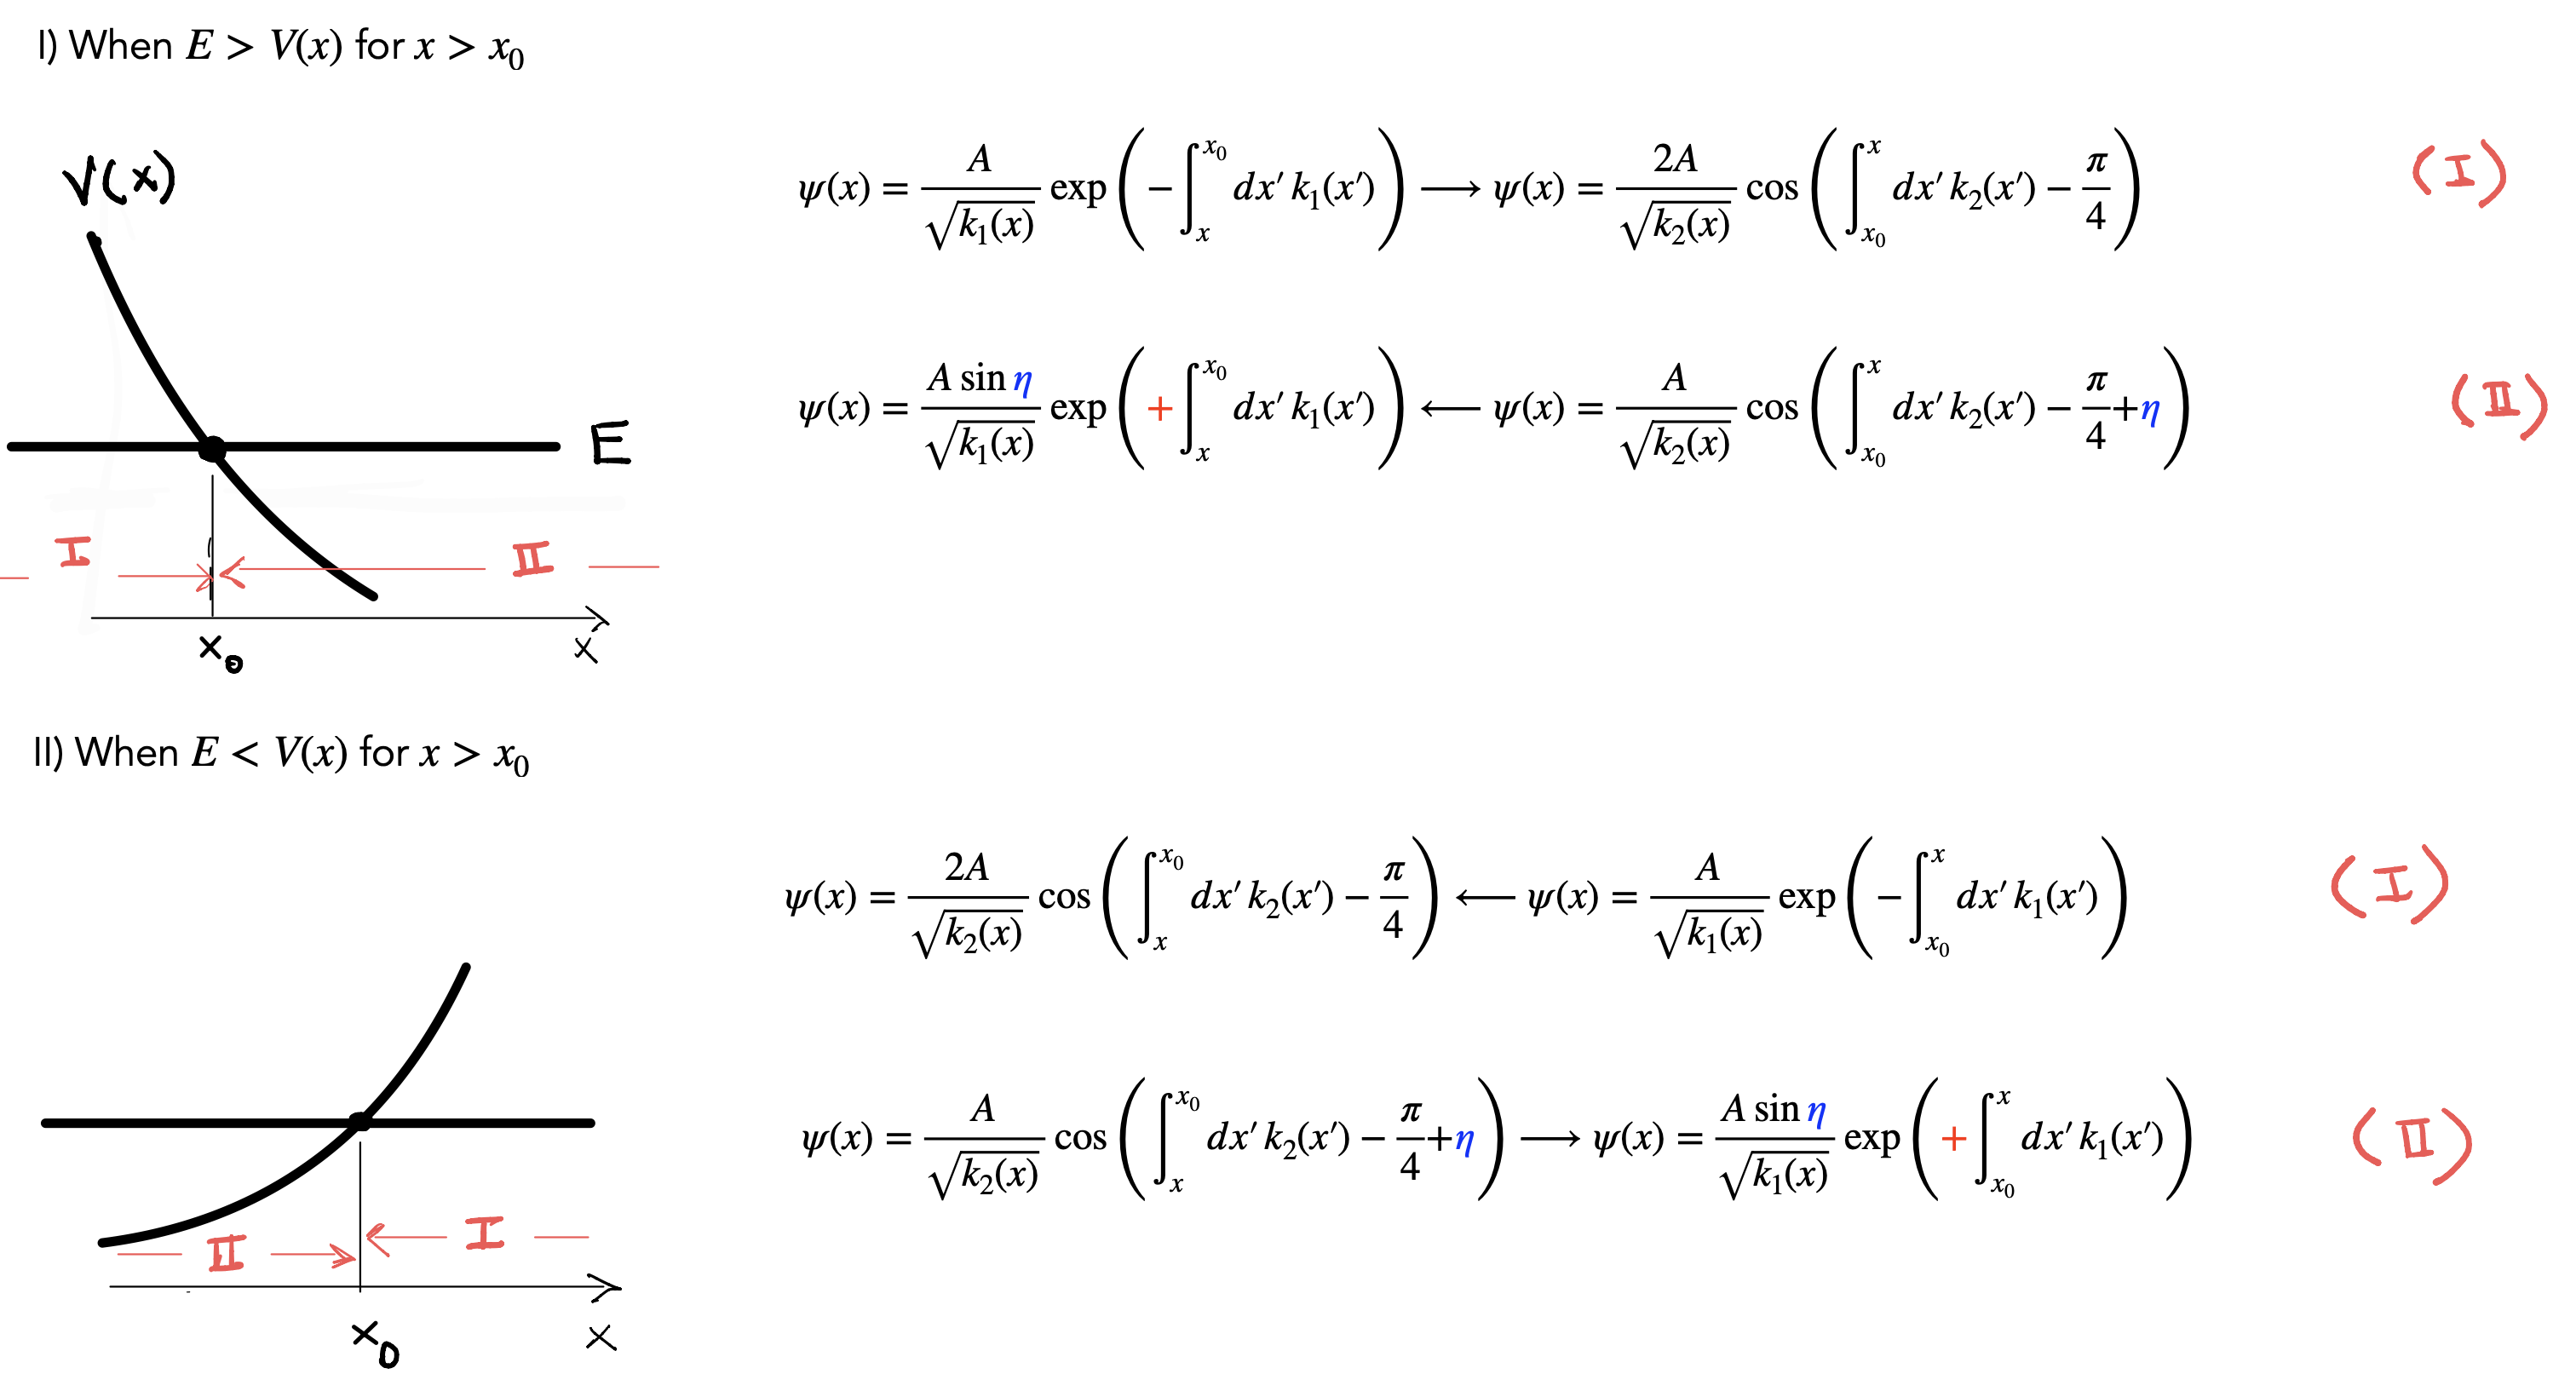
\includegraphics[width=1\linewidth]{src/WKB connection.png}
\end{figure}\end{center}

\subsection{Tunneling}
Consider scattering across rectangular barrier at $[0, L]$ with surrounding $V=0$. 
\[
    \psi(x) = \begin{cases}
        A\exp(ikx) + B\exp(-ikx) & x<0 \\ 
        \displaystyle 
        \df C {\sqrt{|p(x)|}}\exp\left(\df 1 \hb \int_0^x |p(x')|\, dx'\right) + 
        \df D {\sqrt{|p(x)|}}\exp\left(-\df 1 \hb \int_0^x |p(x')|\, dx'\right) & 0<x<L \\ 
        F\exp(ikx) & L<x
\end{cases}\] 
For large barriers, $C$ must be small so the The tunneling probability related 
by the decrease of the exponential decay term across the barrier. 
\begin{mdframed}
    \begin{equation}
        \label{eqn:wkb_tunneling}
        T = \left|\df F A\right|^2 \sim \exp\left(-\df 2 \hb \int_0^L |p(x)|\, dx\right)
    \end{equation}
\end{mdframed}
For general left-incident tunneling with regions $1, 2, 3$ 
being classically allowed, forbidden, and allowed, respectively. 
We have 
\malign{
    \psi_{1}(x) &= A\psi_{\mrm{WKB}, \rightarrow}(x) + B\psi_{\mrm{WKB}, \leftarrow}(x) \\ 
    \psi_{2}(x) &= C\psi_{\mrm{WKB}, \rightarrow}(x) + D\psi_{\mrm{WKB}, \leftarrow}(x) \\ 
    \psi_{3}(x) &= F\psi_{\mrm{WKB}, \rightarrow}(x)\\ 
}
This tunneling formula turns out to be useful not only for barriers with $0$ 
surrounding potentials but also general barriers. 
Using the connection formulas from $3\to 2\to 1$ relates 
$A, B$ as functions of $F$. The transmission coefficient coincides 
with equation~\ref{eqn:wkb_tunneling}. 
However, the reflection coefficient calculates to $R=|B/A|^2=1$. 
This violates the conservation of probability! 
We can only trust equation~\ref{eqn:wkb_tunneling} for $T\ll 1$. 

\subsection{Bound approximations}
The WKB approximation gives us an approximate wavefunction. 
Connection formulas give how approximations change across turning points 
at which a raw approximation would break down. 
Every confining potential possibly yields bound states. 
A consistent, normalizable connection of 3 approximations across 
classical turning points in the regions 
\begin{itemize}
    \item to the left of the confining potential (w.r.t. energy)
    \item inside the confining potential
    \item to the right of the confiniing potential 
\end{itemize}
yields the quantization condition for bound state energy. 

\subsubsection{Two infinite walls}
When there are two infinite vertical walls $x_-, x_+$ 
\begin{mdframed}
\[ 
    \int_{x_-}^{x_+}dx \, \sqrt{2m(E - V(x))} = \pi \hb n, \quad n=1, 2, \cdots 
\] 
\end{mdframed}
We begin by examining first case with two infinite vertical walls. 
Use the WKB approximation~\ref{eqn:wkb_wavefunction} with lower bound at $x_-$, then 
\[ 
    \psi_{\mrm{WKB}}(x_+) = \df 1 {\sqrt{p(x_+)}}
    \left(\alpha_1 \sin \phi(x_+) + \alpha_2\cos\phi(x_+)\right)=0, \quad 
    \phi(x) = \df 1 \hb \int_{x_-}^x p(x')\, dx' 
\] 
We have $\alpha_2=0$ by boundary condition at $x_-$. 
The equation above then yields the desired quantization condition $\phi(x_+) = 0$. 
\begin{example}[finite square well]
    Consider a finite square well with $V(x) -V_0$ in $[0, L]$ and zero elsewhere. 
    Applying the first approximation yields 
    \[ 
        \int_0^L dx\, \sqrt{2m(E + V_0)} = L\sqrt{2m(E + V_0)} = \pi n \hb 
        \implies E = \df{n^2\pi^2\hb^2}{2mL^2} - V_0
    \] 
    This is equivalent to a vertical shift of the infinite square well solution. 
    While there is no single quantitative metric for how good the approximation is 
    (as opposed to energy ratio), we can estimate by the magnitude of the next term in 
    the expansion. 
\end{example}

\subsubsection{One infinite wall}
When there is one infinite vertical wall at $x_-$, a smooth classical turning point at $x_+$
\begin{mdframed}
    \[ 
        \int_{x_-}^{x_+}dx\, \sqrt{2m(E - V(x))} = \pi \hb \left(n + \df 3 4\right), 
        \quad n = 0, 1, 2, \cdots 
    \] 
\end{mdframed}
Begin with an asymptotic formula for the decay on the right side of the potential. 
\[ 
    \psi_{x>x_+}(x) = \df{A}{\sqrt{k_1(x)}}\exp \left(-\df 1 \hb \int_{x_+}^x dx'\, k_1(x')\right)
\] 
Invoke connection at $x_+$ 
\[ 
    \psi_{x_-<x<x_+}(x) 
    = \frac{2A}{\sqrt{k_2(x)}} \cos \left(\df 1 \hb \int_{x}^{x_+} dx' k_2(x') - \frac{\pi}{4\hb } \right)
\] 
The boundary condition that $\psi_{x_-<x<x_+}(x_-)=0$ yields 
\[ 
    \int_{x}^{x_+} dx' k_2(x') = \pi \hb \left(n + \df 3 4\right)
\] 
\subsubsection{Two smooth turning points}
In case of smooth potential with classical turning points at $x_-<x_+$
\begin{mdframed}
    \[ 
        \int_{x_-}^{x_+} dx\, \sqrt{2m(E - V(x))} = \pi \hb \left(n + \df 1 2\right)
        ,\quad n = 0, 1, 2, \cdots 
    \]  
\end{mdframed}
Begin with an asymptotic formula for the decay on the right side of the potential 
\[ 
    \psi_{x>x_+}(x) = \df{A}{\sqrt{k_1(x)}}\exp \left(-\df 1 \hb \int_{x_+}^x dx'\, k_1(x')\right)
\] 
Invoke connection at $x_+$ and manipulate it to fit the connection formula at $x_-$. 
Here we temporarily omit $1/\hb$ to reduce clutter. 
\malign{
    \psi_{x_-<x<x_+}(x) 
    &= \frac{2A}{\sqrt{k_2(x)}} \cos \left( \int_{x}^{x_+} dx' k_2(x') - \frac{\pi}{4} \right) \\ 
    &= \frac{2A}{\sqrt{k_2(x)}} \cos \left( \left(\int_{x_-}^{x_+} - \int_{x_-}^{x}\right)
        dx' k_2(x') - \frac{\pi}{4} \right) \\ 
    &= \frac{2A}{\sqrt{k_2(x)}} \cos \left( \int_{x_-}^{x}dx'\, k_2(x') - \left(\int_{x_-}^{x_+}
        dx' k_2(x') + \frac{\pi}{4}\right)\right) \\ 
    &= \frac{2A}{\sqrt{k_2(x)}} \cos \left( \int_{x_-}^{x}dx'\, k_2(x') - \df \pi 4 - 
        \left(\int_{x_-}^{x_+}dx' k_2(x') - \frac{\pi}{2}\right)\right) \\ 
}
Invoke the connection formula at $x_-$ again with 
\[ 
    \eta =  \frac{\pi}{2\hb} - \df 1 \hb \int_{x_-}^{x_+}dx' k_2(x') 
\] 
In this classically forbidden region, $\psi_{x<x_-}(x)$ must be a decaying function yet 
the connection yields an increasing exponential. This yields the desired quantization 
condition $\sin\eta = 0$,  
\[ 
    \int_{x_-}^{x_+}dx' k_2(x') - \frac{\pi}{2} = n\pi \hb, \quad\quad n=0, 1, 2\cdots
\] 
The other quantization formulas follows from a similar procedure, with infinite vertical 
walls yielding zero boundary condition. 

% \subsection{Tunneling approximations}
% \begin{definition}[tunneling (transmission) coefficient]
%     A plane wave $\exp(-i(2mE) x)$ 
%     with kinetic energy $E$ incident upon a potential barrier in $[0, L]$ scatters with 
%     \malign{
%         \psi(x\leq 0) &= A\exp(ikx) + B\exp(-ikx)  \\ 
%         \psi(x\geq L) &= F\exp(ikx)
%     }
%     The transmission ratio is definined as 
%     \[ 
%         T = \df{|F|^2}{|A|^2}
%     \] 
%     The transmission ratio is defined generally in terms of the 
%     probability current $|J_{x>L}/J_{x<0}|$
% \end{definition}
% The WKB tunning coefficient is only appropriate in the low limit. 
% \leqalign{eqn:wkb_tunneling}{
%     T_{\mrm{WKB}}= \exp\left[-2\int_{x_-}^{x_+} dx\, \sqrt{2m(V(x) - E)}\right]\ll 1
% }

% To compute the tunneling coefficient, we start from the known expression for a 
% single transmitting plane wave traveling to the right from the barrier (which may 
% still be subject to the potential). 
% \malign{
%     \psi_{x>L}(x) 
%     &= \df{A}{\sqrt{k_2(x)}}\exp \left[i\int_L^x dx'\, k_2(x')\right] \\ 
%     &= \df{A}{\sqrt{k_2(x)}}\cos\left[i\int_L^x dx'\, k_2(x')\right] +
%         \df{Ai}{\sqrt{k_2(x)}}\cos\left[i\int_L^x dx'\, k_2(x') - \df \pi 2\right] \\ 
% }
% Recalling the connection formula, let $\eta = \pm \pi / 4$ for the first and second terms, 
% respectively. 
% \malign{
%     \psi_{0<x<L}(x) 
%     &= \df{A \sin (\pi / 4)}{\sqrt{k_1(x)}}\exp\left[\int_x^L dx'\, k_1(x')\right] +
%     \df{Ai\sin(-\pi / 4)}{\sqrt{k_1(x)}}\exp\left[\int_x^L dx'\, k_1(x')\right] \\ 
%     &= \df A {\sqrt{k_1(x)}} \exp\left[-i \df \pi 4 + \int_x^L dx'\, k_1(x')\right] \\ 
%     &= \df A {\sqrt{k_1(x)}} \exp\left[-i \df \pi 4 + \left(\int_0^L - \int_0^x \right)dx'\, k_1(x')\right] \\ 
% }
% Absorb the second integral into the coefficient and apply the connection formula again. 
% \[ 
%     \cdots 
% \] 
% Additionally, the reflection coefficient is $1$, violating $R+T=0$. 
% Therefore equation~\ref{eqn:wkb_tunneling} can only be trusted for $T_{\mrm{WKB}}\ll 1$. 
\section{Scattering}
\subsection{Classical scattering}
In scattering problems, we assume a spatially and temporally uniform distribution of 
incoming beams along the incident axis. We also assume cylindrical 
symmetry parameterized by $(z, b, \phi)$ denoting height, radius, and 
azimuthal angle, respectively. Below are the quantities involved 
in the problem. 
\begin{itemize}
    \item Impact prameter $b$, scattering angle $\theta$.
    \item Particles incident within an infinitesimal patch 
    of cross-sectional area $d\sigma = b\, db\, d\varphi$ scatters into a 
    solid angle (normalized area form) $d\Omega = \sin\theta \, d\theta\, d\varphi$. 
    \item Differential cross-section 
    $d_\Omega \sigma = \df b {\sin\theta}\left|d_\theta b \right|$. 
    Usually, the greater $\theta$ (more pronounced scattering), the smaller $b$, thus 
    the absolute sign. $d_\Omega \sigma$ is usually a 
    quantity parameterized by $\theta$. It asks: at angle $\theta$ 
    from the scattering center, how much unit solid angle accounts 
    for unit area increase in incident beams? 
    \item The total cross-section $\sigma = \int d_\Omega \sigma\, d\Omega$. It is 
    the total cross-sectional area which will encounter scattering. For classical hard-sphere 
    scattering, this is $\pi R^2$. 
    \item The luminosity $\mathcal L$ is the experimentally controllable 
    parameter denoting the number of incident particles 
    per unit cross-sectional area, per unit time. We have 
    $dN = \mathcal L\, d\sigma$, so 
    $d_\Omega\sigma = \df 1 {\mathcal L} d_\Omega N$
\end{itemize}
\begin{figure}[h!] % The [h!] tries to place the figure "here" as closely as possible
    \centering
    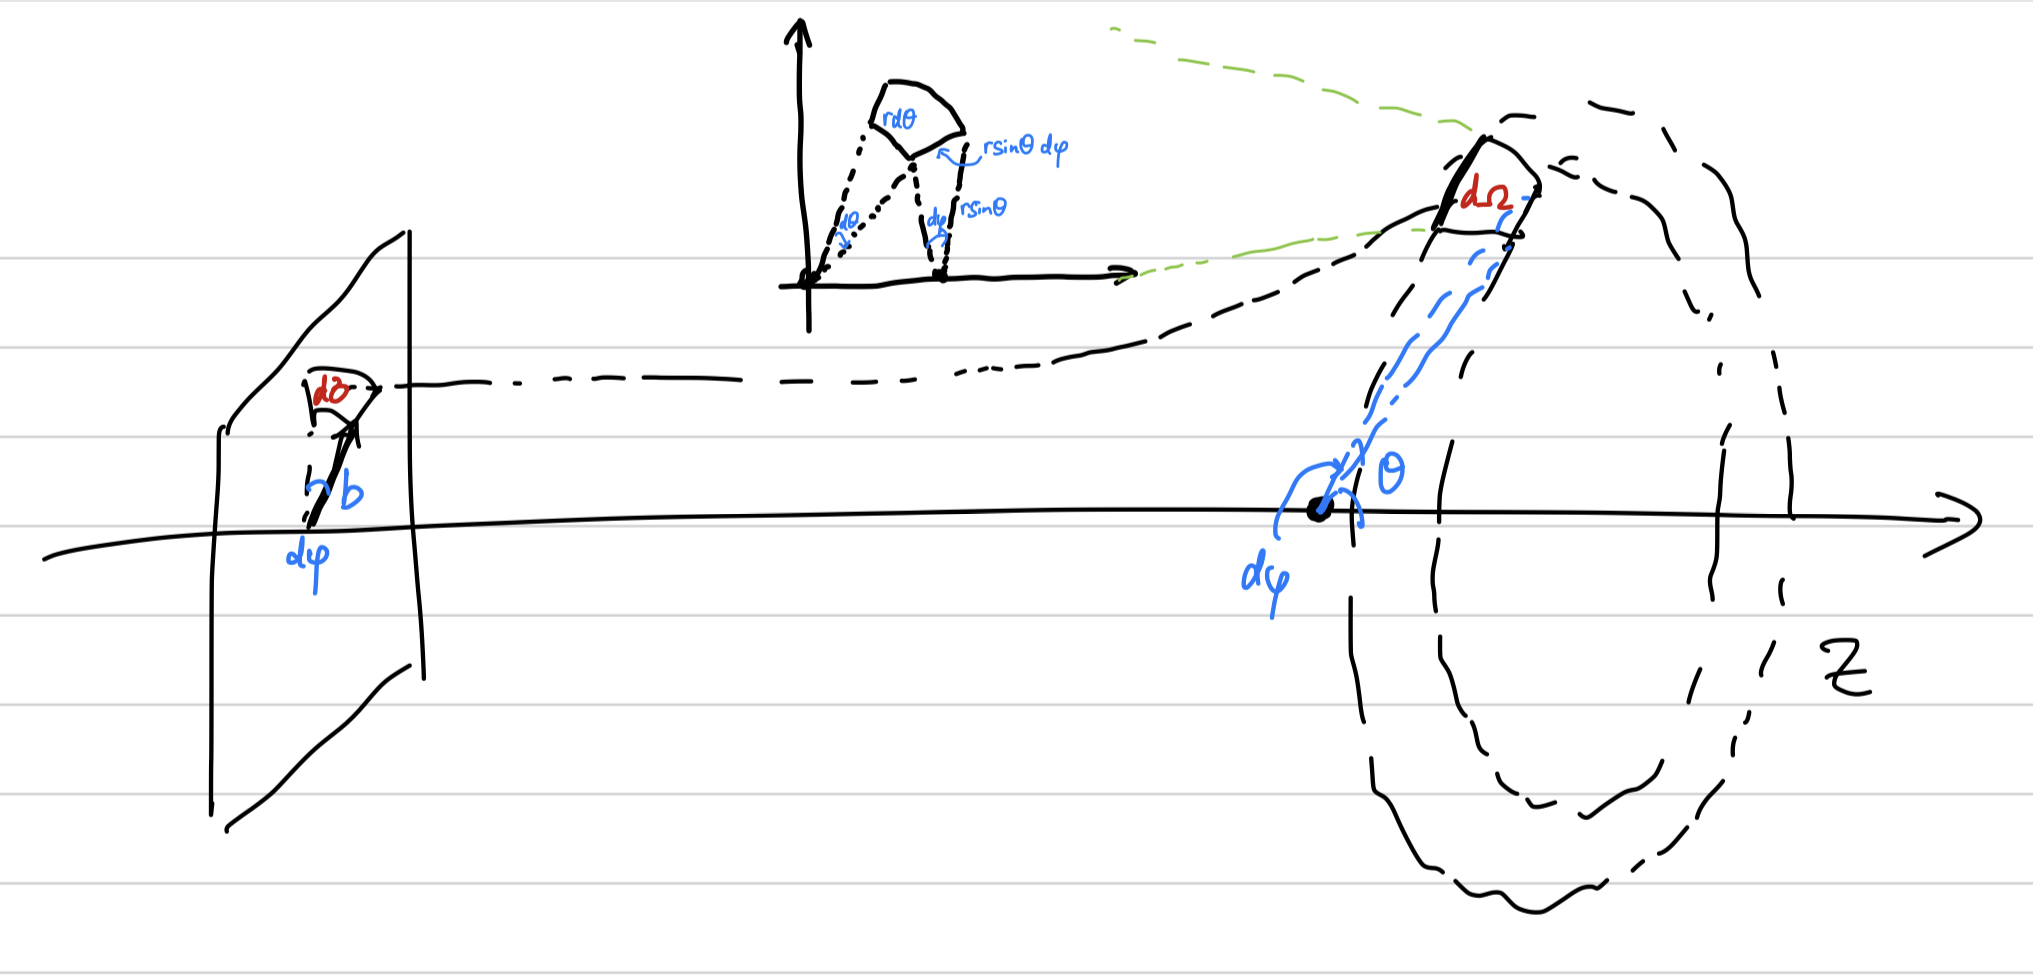
\includegraphics[width=1\linewidth]{src/scattering.jpeg}
    % \caption}
    \label{fig:scattering}
\end{figure}



\subsection{Quantum scattering theory}
Assuming that the scattering potential is localized and spherically symmetric, 
it admits separable solutions 
\[ 
    \psi(r, \theta, \phi) = \sum_{l, m} \df{u_{m, l}(r)}{r} Y^m_l(\theta, \phi)
\] 
Here $u$ satisfies one-dimensional radial equation with effective potential 
\leqalign{eqn:radial se}{
    -\df{\hb^2}{2m} \pd r^2 u + \left[V(r) + \df{\hb^2}{2m} \df{L^2}{r^2}\right]u = Eu 
}
For asymptotically large $kr\gg 1$, the effective potential converges to the radial potential, 
which gives the general solution 
\[ 
    \psi(r, \theta, \phi) = \df{Y^m_l(\theta, \phi)}r\left(Ce^{ikr} + De^{-ikr}\right)
\] 
The outgoing scattering condition eliminates $D$. Our potential starts out 
with both polar and azimuthal symmetry. 
Incidence direction chooses a preferred $z$-axis and 
introduces $\theta$ dependence by breaking spherical symmetry
However, the azimuthally symmetric incidence condition 
leaves our state $\phi$-invariant. 
The only $\phi$-invariant spherical harmonics are those with $m=0$, so 
we look for steady state solutions for $r\gg 1$ of the following form: 
\begin{mdframed}
\leqalign{eqn:radiation state}{
    \psi(r, \theta) = 
    A\left[e^{ikz}+\left(\sum_{l=0}^\infty c_l Y^0_l(\theta)\right)\df{e^{ikr}}{r}\right]
    ,\quad k = \df{2mE}{\hb}
}
\end{mdframed}
The spherically normalized amplitudes in parantheses are collected into the 
\textit{scattering amplitude} $f(\theta)$. 
The probability flux of a uniform 
beam through cross-sectional area $d\sigma$ is 
\[ 
    dP = |\psi_{\mrm{incident}}|^2\, d\sigma = |A|^2 \, d\sigma 
\] 
This is equal to the probability that it scatters into the 
corresponding solid angle $d\Omega$: 
\[ 
    dP = |\psi_{\mrm{scattered}}|^2\, d\Omega = \df{|Af|^2}{r^2} (r^2\, d\Omega)
    = |Af|^2\, d\Omega 
\] 
The differential cross-section is correspondingly 
\[ 
    d_\Omega \sigma = |f(\theta)|^2
\] 
The subsequent subsections introduce two methods to compute the 
scattering amplitudes. 


\subsection{Partial wave analysis}
Partial wave analysis allows us to calculate the scattering amplitudes 
for localized $V(r)$ which \textit{decays faster than $r^2$} 
(this includes finite-range potentials). 

Consider equation~\ref{eqn:radial se} again. 
When $V(r)$ decays faster than $r^{-2}$, our space 
can be split into three regions of interest 
(note that Coulomb potential is not well-localized in this sense). 
\begin{itemize}
    \item scattering region: $V\neq 0$ and $kr\gg 1$. Here a full consideration 
    is needed. 
    \item intermediate region: $V(r)\approx 0$ but the centrifugal term 
    $\df{\hb^2}{2m} \df{L^2}{r^2}$ is still nonneglegible. The particle is radially ``free". 
    \item radiation zone:  $kr\gg 1$, so both $V(r)$ and the centrifugal terms are neglegible. 
    The state in this regime is given by equation~\ref{eqn:radiation state}.
\end{itemize}
We consider the intermediate region, equation~\ref{eqn:radial se} becomes 
\leqalign{eqn:intermediate region se}{
    u(r) = Arj_l(kr) + Brn_l(kr)
}
Here $n_l, j_l$ are the spherical Bessel functions which somewhat represents 
sines and cosines. It is more helpful to change basis to linear combinations 
of the Bessels representing the analogue of complex exponentials, or the 
\textit{spherical Hankel functions} which are asymptotically $e^{\pm ikx}/r$
\[ 
    h_l^{(1)}(x) \equiv j_l(x) + in_l(x), \quad h_l^{(2)}(x) = j_l(x) - in_l(x)
\] 
Outgoing solutions are represented by Hankel functions of the first kind, 
so the intermediate region's state is of the form 
\[ 
    \psi(r, \theta) = A\left[e^{ikz} + \sum c_{m, l} Y^m_l(r, \theta)R_l(r)\right] = 
    A\left[e^{ikz} + \sum_{l=0}^\infty c_l h_l^{(1)}(kr) Y_l^0(\theta)\right]
\] 
Redefine expansion coefficients with the \textit{$l$-th partial wave 
amplitude} $c_l = i^{l+1}k\sqrt{4\pi(2l+1)}a_l$; this parameterization turns 
out to be useful later. Substituting $Y_l^0(\theta)$ yields 
\[ 
    \psi(r, \theta) = A\left[e^{ikz} + 
    k\sum_{l=0}^\infty i^{l+1}(2l+1)a_lh^{(1)}_l(kr) P_l(\cos\theta)\right]
\] 
To use consistent spherical coordinates, we need to use Rayleigh's formula 
\leqalign{eqn:Rayleigh's formula}{
    e^{ikz} = \sum_{l=0}^\infty i^l(2l+1)j_l(kr)P_l(\cos\theta)
}
The intermediate region's state is then of the form 
\begin{mdframed}
    \leqalign{eqn:intermediate region se}{
        \psi(r, \theta) = A
        \sum_{l=0}^\infty i^{l}(2l+1)\left[j_l(kr) 
        + i k a_lh^{(1)}_l(kr)\right] P_l(\cos\theta)
    }
    \end{mdframed}
The $l$-th partial wave amplitudes $a_l$ are so defined because for 
large $r$, the Hankel functions approach $(-i)^{l+1}e^{ikr}/kr$, so 
equation~\ref{eqn:intermediate region se} approaches 
equation~\ref{eqn:radiation state} with 
\[ 
    f(\theta) = \sum_{l=0}^\infty c_l Y^0_l(\theta)
    = \sum_{l=0}^\infty (2l+1)a_lP_l(\cos\theta)
\] 
The differential cross-section can be computed from the partial wave amplitudes by 
\leqalign{eqn:quantum differential cross section}{
    d_\Omega \sigma(\theta) = |f(\theta)|^2 = 
    \sum_{l, l'}(2l+1)(2l'+1)a_l^*a_{l'}P_l(\cos\theta)P_{l'}(\cos\theta)
}
Integrate over the solid angle to obtain the total cross section 
\leqalign{eqn:quantum total cross section}{
    d_\Omega \sigma(\theta) = |f(\theta)|^2 = 
    4\pi \sum_{l=0}^\infty (2l+1)|a_l|^2
}
When the centrifugal term dominates over the radial potential, 
the partial wave components are dominated by components with low angular 
momentum. 

For an algorithmic prescription of partial wave analysis: 
\begin{itemize}
    \item Choose a potential cutoff $R$ beyond which to use 
    equation~\ref{eqn:quantum differential cross section}. 
    Solve for the eigenstates of the potential for $r\leq R$. 
    \item Use matching boundary conditions to evaluate $a_l$. 
    \item Use the partial wave amplitudes to calculate quantities of interest. 
    If possible, for infinite-range but quickly-decaying potentials take $R\to \infty$. 
\end{itemize}


% \subsection{Phase shifts}
% The whole story simplifies considerably when the potential is spherically 
% symmetric. This implies that angular momentum is conserved and each partial wave 
% below is independently scattered with no change in amplitude, only in phase. 
% We consider this rigorously 
% \[ 
%     \psi^{(l)} = A i^l(2l+1)j_l(kr)P_l(\cos\theta), \quad V(r) = 0
% \] 
% For large $r$, this takes the asymptotic form 
% \[ 
%     \psi^{(l)} \approx A\df{(2l+1)}{2ikr}\left[e^{ikr} - (-1)^l e^{-ikr}\right]P_l(\cos\theta)
% \] 

\subsection{Integral form of the eigenvalue equation}
The three-dimensional eigenvalue equation for the Hamiltonian may be rewritten as 
\leqalign{eqn:3d se}{
    (\nabla^2 + k^2)\psi(\mbf r) = \df{2m}{\hb^2}V(\mbf r)\psi(\mbf r), 
    \quad k = \df{\sqrt{2mE}}{\hb}
}
This has the superficial apearance of a Helmholtz equation
\[ 
    \left(\nabla^2 + k^2\right)\psi = Q, \quad Q(\mbf r) = \df{2m}{\hb^2}V(\mbf r)\psi(\mbf r)
\] 
However, the important difference is that the inhomogeneous term $Q$ 
now also depends on $\psi$. Recall that given a 
Green function $G(\mbf r)$ which solves the Helmholtz equation with a 
delta function ``source'', integrating it gives the solution 
to the Helmholtz equation. 
\leqalign{eqn:green condition}{
    (\nabla^2 + k^2)G(\mbf r) = \delta^3(\mbf r)
}
While a Green function will not allow us to write the closed form 
to the eigenvalue equation, it yields an equivalent equation 
(note that $\psi$ also appears on the right hand side). 
\[ 
    \psi(\mbf r) = \int d^3\mbf r' \, 
    Q(\mbf r') G(\mbf r - \mbf r')
\] 
To see that this equation is equivalent to equation~\ref{eqn:3d se}, 
apply $(\nabla^2+k^2)$ to both sides. 
\[ 
    (\nabla^2 + k^2)\psi(\mbf r) = 
    \int d^3\mbf r'\left(\nabla^2 + k^2\right)G(\mbf{r - r'}) Q(\mbf r') 
    = \int \delta(\mbf{r-r'})Q(\mbf r')\, d^3\mbf r' = Q(\mbf r)
\] 
One Green function which satisfies equation~\ref{eqn:green condition} is 
\[ 
    G(x) = -\df{e^{ikr}}{4\pi r}
\] 
The free part of the eigenvalue equation solution is the kernel 
of $\nabla^2+k^2$ corresponding to the free-particle solutions. 
This allows us to write the general integral form of equation~\ref{eqn:3d se}. 
\begin{mdframed}
\leqalign{eqn:integral se}{
    \psi(\mbf r) = \psi_0(\mbf r) - 
    \df{m}{2\pi \hb^2}\int \df{e^{ik|\mbf r - \mbf r'|}}{|\mbf r - \mbf r'|}
    V(\mbf r')\psi(\mbf r')d^3\mbf r', \quad  (\nabla^2+k^2)\psi_0(\mbf r) = 0
}\end{mdframed}


\subsection{Born Approximation}
Suppose $V$ is localized about $\mbf r'=0$ 
and we wish to calculate $\psi(\mbf r)$ for points far away from the scattering center. 
The contributing terms all satisfy $|\mbf r'|\ll |\mbf r|$, so 
\[ 
    |\mbf r - \mbf r'| \approx r - r'\cos\theta = r - \hat {\mbf r} \cdot \mbf r'
\] 
\begin{figure} % The [h!] tries to place the figure "here" as closely as possible
    \centering
    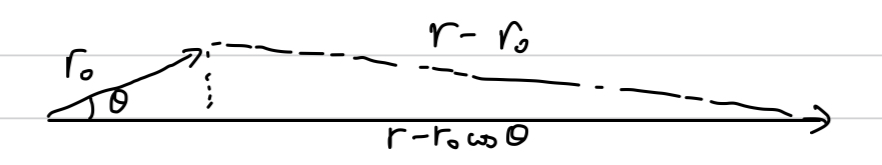
\includegraphics[width=0.5\linewidth]{src/vector difference approx.jpeg}
    \caption{Intuition for $|\mbf r - \mbf r'|\approx r - r'\cos\theta$}
    \label{fig:vector difference approx}
\end{figure}
This is an approximation up to the first order of $r'/r$. 
Let $\mbf k = k\hat r$, then 
\[ 
    e^{ik|\mbf r - \mbf r'|} \approx e^{ikr}e^{i\mbf{k\cdot r'}} 
    \implies \df{e^{ik|\mbf{r - r'}}|}{|\mbf{r-r'}|} \approx 
    \df{e^{ikr}}{r}e^{-i\mbf{k\cdot r'}} 
    % \approx \df{e^{ikr}}{r}\left(1 - i\mbf k\cdot \mbf r'\right)
\] 
Substituting into equation~\ref{eqn:integral se} with the free 
solution $\psi_0=e^{ikz}$ reads 
\leqalign{eqn:far born integral}{
    \psi(\mbf r) \approx e^{ikz} - 
    \df{m}{2\pi \hb^2} \df{e^{ikr}}{r}\int e^{-i\mbf{k\cdot r'}}
    V(\mbf r')\psi(\mbf r')\, d^3\mbf r'
}
Equation~\ref{eqn:far born integral} is ``exact'' to the first 
order in $r'/r$, so it is actually exact for the purposes of calculating the 
scattering amplitudes, which are at asymptotically large $r$. 
Equation~\ref{eqn:far born integral} 
standard form of the eigenstate in the radiation zone. 
Recall from~\ref{eqn:radiation state} that the scattering amplitudes 
are the coefficients of $Ae^{ikr}/r$ at large $r$, we 
can read off their \textit{exact} values 
\leqalign{eqn:wave amplitude equation}{
    f(\theta, \phi) = -\df{m}{2\pi \hb^2A}\int e^{-i\mbf{k\cdot r'}}V(\mbf r')\psi(\mbf r')d^3\mbf r'
}
Note that the right hand side contains $\psi$ so this is not a closed form. 
The Born approximation assumes that the incoming 
wave is not substantially altered by the scattering, 
so 
\[ 
    \psi(\mbf r')\approx \psi_0(\mbf r') = Ae^{ikz'} = Ae^{i\mbf k'\cdot \mbf r'}, \quad \mbf k' = k\hat z 
\] 
This yields the first Born approximation for scattering amplitudes. 
The following holds when \textit{the incident energy is large compared to the potential}. 
\begin{mdframed}\leqalign{eqn:first born approximation}{
    f(\theta, \phi) \approx -\df{m}{2\pi \hb^2} 
    \int e^{i\mbf{(k' - k)\cdot r'}}V(\mbf r')d^3\mbf r', \quad \mbf k' = k\hat z, \mbf k = k\hat r_{\theta, \phi}
}\end{mdframed}
Note that $\mbf k'$ points in the direction of the incident beam, 
while $\mbf k$ points in the scattering direction. 
Additionally, \textit{when the energy of the incident beam is low} 
so that the wavelength is large compared to the 
scattering region, $e^{i\mbf{(k-k')\cdot r'}}$ is essentially constant over $\mbf r'$ 
for which $V(\mbf r')$ is significant, in which case 
\leqalign{eqn:low energy born approx}{
    f(\theta, \phi) \approx -\df{m}{2\pi \hb^2}\int V(\mbf r')\, d^3\mbf r'
}
When the potential is spherically symmetric, the first 
Born approximation~\ref{eqn:first born approximation}
may be explicitly evaluated. The following equation does not require low incident energy, 
only the Born condition that the incident energy is large compared to the potential. 
\begin{mdframed}
    \leqalign{eqn:spherical low energy born approx}{
        f(\theta) \approx -\df{2m}{\hb^2\kappa} \int_0^\infty rV(r)\sin(\kappa r)\, dr, 
        \quad \kappa = 2k\sin(\theta/2)
    }    
\end{mdframed}
\section{Second Quantization}
This section uses Chapter 2 of~\cite{altland2010condensed} 
available \href{https://www.tcm.phy.cam.ac.uk/~bds10/tp3/secqu.pdf}{here} and 
these \href{https://ethz.ch/content/dam/ethz/special-interest/phys/theoretical-physics/cmtm-dam/documents/qg/Chapter_05-06.pdf} 
{lecture notes} from ETH. 

Particles belong to one of two indistinguishable classes: fermions or bosons, which are 
antisymmetric and symmetric under particle exchange, respectively. Instead of explicitly 
symmetrizing a wave function, we can instead adapt our mathematical formulation to 
inherently account for indistinguishability and even varying number of particles. 

\begin{definition}[occupation number state]
    The occupation number state $|n_1, \cdots\ra$ denotes $n_i$ fermion or bosons 
    in level $i$. The total number of particles is given by 
    \[ 
        N = \sum n_i 
    \] 
    The space of all occupation number states for all $N$ is called Fock space. 
    Explicitly, let $S_\pm$ denote the (anti)-symmetrizer 
    \[ 
        S_\pm |i_1, \cdots, i_N\ra = \df 1 {N!} \sum_{P\in S_N} \sgn(P)\,  P|i_1, \cdots, i_N\ra 
    \] 
    the occupation state is $|n_1, \cdots\ra_{\pm} = S_\pm |i_1, \cdots, i_N\ra$ 
\end{definition}
\begin{proposition}
    $\la n_1, \cdots|n'_1\cdots\ra = \prod \delta_{n_i, n'_i}, \quad 
    \sum_{n_1, \cdots}|n_1, \cdots\ra \la n_1, \cdots| = 1$
\end{proposition}
\begin{definition}[creation and annihilation operators]
    The creation and annihilation operators $a_i^\dag, a_i$ of a particle 
    in level $i$ is defined to be 
    \malign{
        a_i^\dag |\cdots, n_i, \cdots\ra = \sqrt{n_i+1}|\cdots, n_i+1, \cdots\ra \\ 
        a_i|\cdots, n_i+1, \cdots\ra = \sqrt{n_i+1}|\cdots, n_i, \cdots\ra 
    }
    the second equation follows from the first by the adjoint definition. 
\end{definition}
\begin{theorem}[commutation relations]
    Consistent symmetrization implies 
    \begin{flalign*}
        && [a_i, a_j] &= [a_i^\dag, a_j^\dag] = 0, \quad [a_i, a_j^\dag] = \delta_{ij}I && \text{(bosons)} \\ 
        && \{a_i, a_j\} &= \{a_i^\dag, a_j^\dag\} = 0, \quad \{a_i, a_j^\dag\} = \delta_{ij}I && \text{(fermions)}
    \end{flalign*}
    They are called the canonical commutation relations (CCRs). 

    \prf we consider the fermions first. Given $|n_1, \cdots\ra=S_-|i_1, \cdots, i_N\ra$, we have 
    \malign{
        a_k^\dag a_j^\dag |n_1, \cdots\ra &= S_-|i_1, \cdots, i_N, j, k\ra  \\ 
        a_j^\dag a_k^\dag |n_1, \cdots\ra &= S_-|i_1, \cdots, i_N, k, j\ra 
    }
    Now they differ by a sign since $|i_1, \cdots, i_N, j, k\ra, |i_1, \cdots, i_N, k, j\ra$ 
    differ by a transposition $(N+1, N_2)$, so $\{a_i^\dag, a_j^\dag\}=0$. 
    Further note that antisymmetrization annihilates a vector if it contains any duplicate 
    basis, so $n_i=0, 1$. We omit the rest of the proof. 
\end{theorem}
\textbf{todo}
\begin{corollary}
    For fermions, the CCRs imply 
    \begin{flalign*}
        && a_j^2 = (a_j^\dag)^2 = 0,& \quad a_ja_j^\dag = I - a_j^\dag a_j \\ 
        && a_ja_k^\dag = -a_k^\dag a_j,& \quad a_ja_k = -a_ka_j && j\neq k
    \end{flalign*}
    For bosons, 
    \begin{flalign*}
        a_ja_j^\dag = I + a_j^\dag a_j, \quad a_ja_k^\dag = a_k^\dag a_j, \quad a_ja_k = a_ka_j
    \end{flalign*}
\end{corollary}
Let $V$ be the Hilbert space of one particle, then the occupation (Fock) space 
is $\mca F \cong V^0\oplus V^1\oplus V^2\oplus \cdots$. 
\begin{definition}[vacuum and general states]
    The vacuum state, denoted $|0\ra$ or $|\Omega\ra$, is the state annihilated by all annihilation operators. 
    One can also explicitly write out the occupation number state, for $\zeta=\pm 1$ denoting bosons 
    and fermions, respectively 
    \[ 
        |(n_i)\ra = \df 1 {\sqrt{\prod (n_i!)}} \left[\prod (a_i^\dag)^{n_i}\right]|\Omega\ra 
    \] 
\end{definition}
\begin{corollary}
    Pauli exclusion principle: for fermions $(a_i^\dag)^2=0$.  
    No single particle state can be occupied by more than one fermion. 
\end{corollary}
\begin{definition}[occupation number operator]
    the occupation number operator is the Hermitian operator defined by 
    \[ 
        N_i = a_i^\dag a_i, \quad N_i|(n_i)\ra = n_i |(n_i)\ra 
    \] 
    For both fermions and bosons, it satisfies 
    \[ 
        N_j (a_j^\dag)^n|\Omega\ra = n (a_j^\dag)^n|\Omega\ra, \quad [N_j, a_{k\neq j}^{(\dag)}]=0
    \] 
    The total particle number operator is 
    \[ 
        N = \sum a_i^\dag a_i 
    \] 
\end{definition}
Note that the level index $i$ implicitly assumes a basis (e.g. position or momentum, 
or spin along a particular direction). Suppose we wish to change into another basis $j$. 
\begin{proposition}
    change of basis formula $a^\dag_j = \la i|j\ra a_i^\dag, a_j = \la j|i\ra a_i$. 

    \prf note that single kets $|i\ra = a_i^\dag |\Omega\ra$. Then $|j\ra = a_j^\dag|\Omega\ra $, then 
    \[ 
        |j\ra = \la i|j\ra |i\ra = \la i|j\ra (a_i^\dag |\Omega) = a_j^\dag |\Omega\ra 
    \] 
\end{proposition}
\begin{proposition} the second quantization of a single-particle operator $O\in \End(V)$ is 
    \[ 
        O = \la i|O|j\ra a_i^\dag a_j 
    \] 
    
    \prf 
    Suppose $O$ is a single-particle operator with eigenbasis $o_\lambda, |\lambda\ra$. 
    In the second-quantization scheme, it has the representation 
    \[ 
        O = o_\lambda n_\lambda 
    \] 
    In other words, it counts how many particles are in each of the $|\lambda\ra$ eigenstates and 
    assigns the proper weights to them. Using a change of basis into arbitrary basis indexed by $i$ 
    or $j$ 
    \[ 
        o_\lambda n_\lambda 
        = \la \lambda|O|\lambda\ra a_\lambda^\dag a_\lambda 
        = \la \lambda|O|\lambda\ra \la i|\lambda\ra \la \lambda |j\ra a_i^\dag a_j \\ 
        = \la i|O|j\ra a_i^\dag a_j 
    \] 
\end{proposition}
We next consider the second quantization of two-body interaction operators. 
\begin{proposition}
    $V = \la i, j|V|k, l\ra a_i^\dag a_j^\dag a_ka_l$ 
\end{proposition}
\begin{definition}[field operators]
    Let $|\br\ra$ denote a particle localized at $\br$. This constitutes a special 
    basis. Given creation and annihilation operators in some basis indexed by $i$, denote 
    \[ 
        \la \br|i\ra = \phi_i(\br)
    \] 
    the creation and annihilation operators in the position basis, are called 
    the field operators 
    \[ 
        \hat \psi^\dag(r) = \phi_i^*(\br)a_i^\dag 
    \] 
\end{definition}
\end{document}
